% 下面这句用以支持中文
% !Mode:: "TeX:UTF-8"

%%% Local Variables:
%%% mode: latex
%%% TeX-master: t
%%% End:

\chapter{ISSD信息传播结构多样化模型}
\label{cha:5thChap05}

\section{引言}
近年来,信息传播是复杂网络传播动力学研究的热点之一,特别是随着社交网络的爆炸式发展,越来越多的人开始利用微博、微信、人人网等来传播信息、分享趣事和观点,这为研究信息传播提供了前所未有的实际数据。信息传播对于新思想、新技术、新产品等带来了无限的商机与机遇,同时也对社会稳定造成了极大的危害,甚至引发社会动荡,这给谣言控制、舆情监控、信息引导提出了新的挑战。因此,研究信息传播具有极其重要的理论与现实实际意义。

目前信息传播研究,从宏观角度分析,主要基于传染病传播的研究框架模型,参照第~\ref{SIModel}节,考虑了信息传播的部分特征,进行了建模分析,但是忽略了传播者的个体差异,及信息传播与传染病传播完全不同的独有特性;从微观角度分析如独立级联模型(IC),具体参照第~\ref{chap2:ICModel}节,和线性阈值模型(LT),具体参照第~\ref{chap2:LTModel}节,但是没考虑信息传播者的外部环境影响因素和随时间变化等因素。虽然目前研究人员开始广泛聚焦信息传播研究,但是信息传播是个及其复杂的过程,新媒体下信息传播的模型是什么?其传播特征规律是什么?如何刻画信息传播随时间动态演化的过程?等等,依然是一个个待深入研究的重要内容。本章重点从微观结合中观的层次角度进行分析,探索信息传播的模型与规律特点。


\section{相关工作}
目前,越来越多的用户应用社交网络传播信息、分享信息。如腾讯微信、新浪微博等成为人们获取信息的重要渠道来源、交互信息的重要平台和共享信息的载体。信息在社交网络上传播是一个相当复杂的过程,除了涉及到个人用户的认知心理、个人喜好、个人知识背景等个体属性因素,还会受所在的社交圈子、朋友之间的关系程度,以及整个社会大环境对相关话题的关注程度等,这些外部环境因素的多方面影响。在已有的相关研究中,信息传播常建立在传染病模型基础上进行宏观分析。文献\cite{huang2011preventing}利用SIS的信息传播模型,研究了谣言的传播过程,文献\cite{zhao2012sihr}提出了SIHR模型,也分析了谣言的规律。文献\cite{zhangyancao2011}利用传染病动力学理论分析了信息传播的SIR模型。Anderson等人\cite{anderson1991infectious}提出了SEIR模型,在经典的SIR模型中增加了潜伏节点E(Exposed)。文献\cite{lu2011small}也利用传染病模型分析了信息在规则网络、小世界网络中的传播规律,并归纳了信息传播的一些特点,这些信息传播的研究给我们提供了很好的参考依据。但上述基于传染病传播模型的信息传播方法,只是从整体角度分析了传播规律,没有考虑到每个人用户(节点)的个体差异,及信息随时间变化的特有规律,因为信息传播与传染病传播是有本质不同的。Ugander等人\cite{ugander2012structural}利用实际Facebook真实数据,实际分析了社交网络中用户接受信息具有的结构多样性的特点。如用户从两个不同圈子听到一条信息其可信程度要远远高于从一个圈子内听到两次。其过程分析如图~\ref{fig:DSpnas2012}所示。这篇文章使用相对转化率(Relative conversion rate)代表个体被说服注册Facebook的可能性大小。首次观测了邻居的数目和邻居连通子图对相对转化率的影响,文章详细列出了2、3、4个邻居的用户的相对转化率的情况。从下面的图中可以看出,固定邻居数量,在连通子图的数目相同时,不同连接情况下的转化率相差不大,但是当连通子图数目增大时,转化率会有相当大的提升。
\begin{figure}[H] % use float package if you want it here
	\centering
	\includegraphics[scale=0.9]{./chap5/SDpnas2012}
	\caption{Facebook中结构多样性对用户转化分析情况\cite{ugander2012structural}}
	\label{fig:DSpnas2012}
\end{figure}

%\subsection{overlap}
%\subsubsection{community}
%\subsubsection{community}
%\subsection{unoverlap}
%\subsubsection{clique}
%\subsubsection{k-trussess}
%\subsubsection{connect component}
\subsection{信息传播时间变化模型}
%信息衰减函数(newton cool)
信息传播随着时间的变化非常地快,我们参照参考文献\cite{yang2011patterns}中对社交网络Twitter一些热点词及标签内容随时间的变化进行分析,如图~\ref{fig:chap05WSDM11Wang}如示。新信息在产生后迅速传播成为热点信息,然后随着时间快速衰减,成为过时信息。
\begin{figure}[H] 
	\centering
	\includegraphics[scale=0.34]{./chap5/WSDM11Wang}
	\caption{Twitter中某些信息被关注提及随时间的变化规律}
	\label{fig:chap05WSDM11Wang}
\end{figure}
我们从 Alex Bentley等人\cite{bentley2011ll}书中可以知道人们接受一些行为是如何由一小部分热衷创新、学习的人发起,到后来怎么被大众模仿传播开来的。其中有两个重要模式:个人学习模式、模仿学习(社会学习)模式,不同模式下的接受率不同,如图~\ref{fig:chap05IwillhaveWhate}所示,不同的学习模式接受率的增幅变化是不同,这与我们对信息传播受内因、外因共同影响的思路是一致的。
\begin{figure}[H] 
	\centering
	\includegraphics[scale=0.6]{./chap5/chap05IwillhaveWhate}
	\caption{社会信息在个人学习、模仿学习模式下的接受规律}
	\label{fig:chap05IwillhaveWhate}
\end{figure}
%http://www.alex-bentley.com/books
我们也对关键词“环境污染”、“雾霾”及“caijing”应用Google趋势进行统计分析。从图~\ref{fig:chap05Haze1}可以看出“环境污染”2005年大家高度关注,随着时间关注度逐渐下降。由于2015年2月柴静关于雾霾的新闻报告《穹顶之下》又一次爆发成为人们关注的焦点,如图~\ref{fig:chap05Haze2}所示。所以我们识为信息传播不但与用户节点的邻居节点结构多样化的内部环境相关,而且与整个网络外部信息大环境相关,同时我们可以看到人们对信息的关注度随时间变化非常迅速。
\begin{figure}[H] 
	\centering
	\includegraphics[scale=1.0]{./chap5/Haze1}
	\caption{关键词在2004年-2015年3月被关注度随时间的变化趋势}
	\label{fig:chap05Haze1}
\end{figure}
\begin{figure}[H] 
	\centering
	\includegraphics[scale=1.0]{./chap5/Haze2}
	\caption{关键词在2015年2月-2015年3月被关注度随时间的变化趋势}
	\label{fig:chap05Haze2}
\end{figure}

根据以上相关分析,我们可以知道信息传播具有活性,其活跃程度会随外界整个信息大环境影响,且变化很快。我们参照物理学中的"牛顿冷却定律"(Newton's Law of Cooling)\cite{winterton1999newton,incropera2011fundamentals}对信息传播变化进行了相应的建模。牛顿冷却定律是:物体温度变化与外界的温差成正比,如公式:
\begin{equation} 
\label{chap05newtoncool}
T'(t) = -\alpha (T(t)-H) ,\alpha > 0
\end{equation}
其中$\alpha$ 负表示当物体自身温度高于外界温度,相反外界温度大于物体温度,物体温度会升高。如图~\ref{fig:chap05newtonTemp}所示。
\begin{figure}[H] 
	\centering
	\includegraphics[scale=1]{./chap5/newtonTemp}
	\caption{牛顿冷却定律中物体温度随外界温度变化情况}
	\label{fig:chap05newtonTemp}
\end{figure}

我们对应建立信息随时间变化的数学模型--信息传播时间变化模型,用户(个体)对信息感兴趣程度与用户周围邻居知道信息所占比例成正比。可以表示为:
%比例参照2002 watts
\begin{equation} 
\label{chap05infocool}
I'(u,t) = -\rho (I(u,t)-H(u))
\end{equation}
其中$H(u)$为用户$u$对某类信息感兴趣程度,根据实际个体情况设定初始阈值,$I(u,t)$为用户$u$在时间$t$时对某个信息的感兴趣程度;$\rho $ 为兴趣变化参数,如果用户对某信息的兴趣度大于外界信息热度,$\rho \geq 0$,否则相反,人们会对某个信息随时间的变化,进行信息过滤衰减。人们对信息的兴趣随时间变化过程如图~\ref{fig:chap05infoNewton}所示,从图~\ref{fig:chap05infoNewton}上变化的简单曲线可以理解新产品、新技术、新思想的传播趋势走向。虽然这些变化曲线并不能解释一切传播现象,但是我们能够根据一些信息传播的特点作出具体、有用的假设,再进行采样校正,进一步细化,达到传播趋势分析精确化。
\begin{figure}[H] % use float package if you want it here
	\centering
	\includegraphics[scale=2.0]{./chap5/infoNewton}
	\caption{用户节点对某个信息感兴趣随时间变化规律}
	\label{fig:chap05infoNewton}
\end{figure}

对~\ref{chap05infocool}解不定积分推导过程如下:
\begin{equation} 
\label{chap05infocooldirivation}
\begin{split}
&\int \frac{I'(u,t)}{I(u,t)-H(u)} = \int (-\rho)dt \\
&\rightarrow \log |I(u,t)-H(u)| = -\rho t + c \\
&\rightarrow |I(u,t)-H(u)| = C \exp ^{-\rho t }
\end{split}
\end{equation}

\subsection{信息传播结构多样性}
信息传播过程中,用户接受信息受其所在外部环境的影响,即用户的自我网络环境(Egocentric network,简称为Ego网络)\cite{marsden2002egocentric,fisher2005using,weng2014topic}结构多样性对接受信息的影响。Ego网络是整个关系网络的子图,包括一个中心节点和其邻居节点,边包括中心节点与邻居节点,及其邻居节点之间的连线。如图~\ref{fig:chap05SD1}所示,以节点32中心的Ego网络。

\begin{figure}[H]
	\centering%
	\subcaptionbox{节点32的Ego图\label{fig:chap05SD1}}
	%标题的长度,超过则会换行,如下一个小图。
	{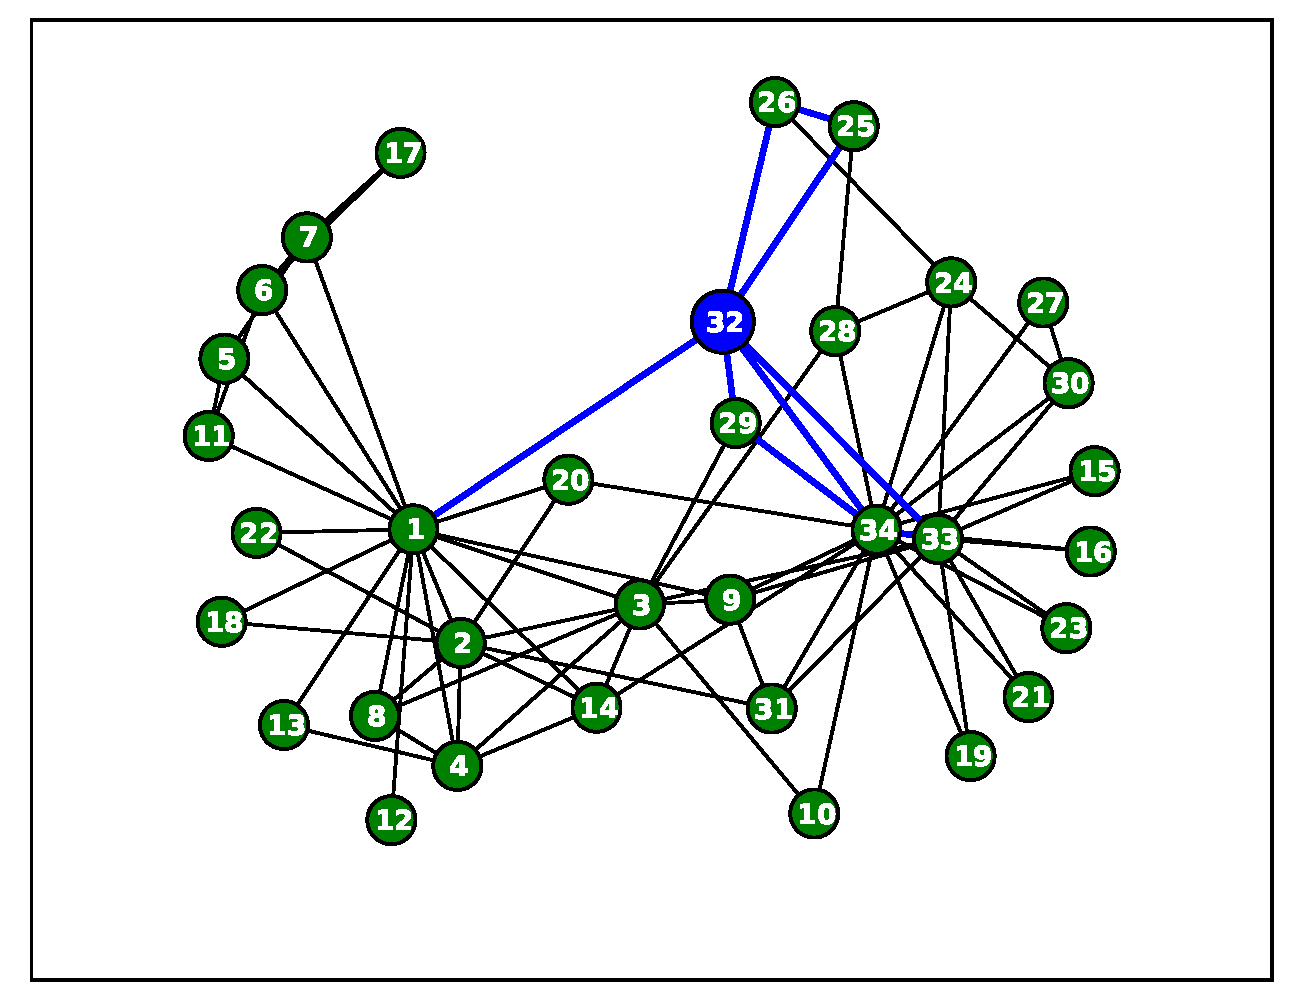
\includegraphics[scale=0.36]{./chap5/SD1}}
	%\hspace{3em}%
	\subcaptionbox{节点32邻居知道某个信息的环境\label{fig:chap05SD2}}
	{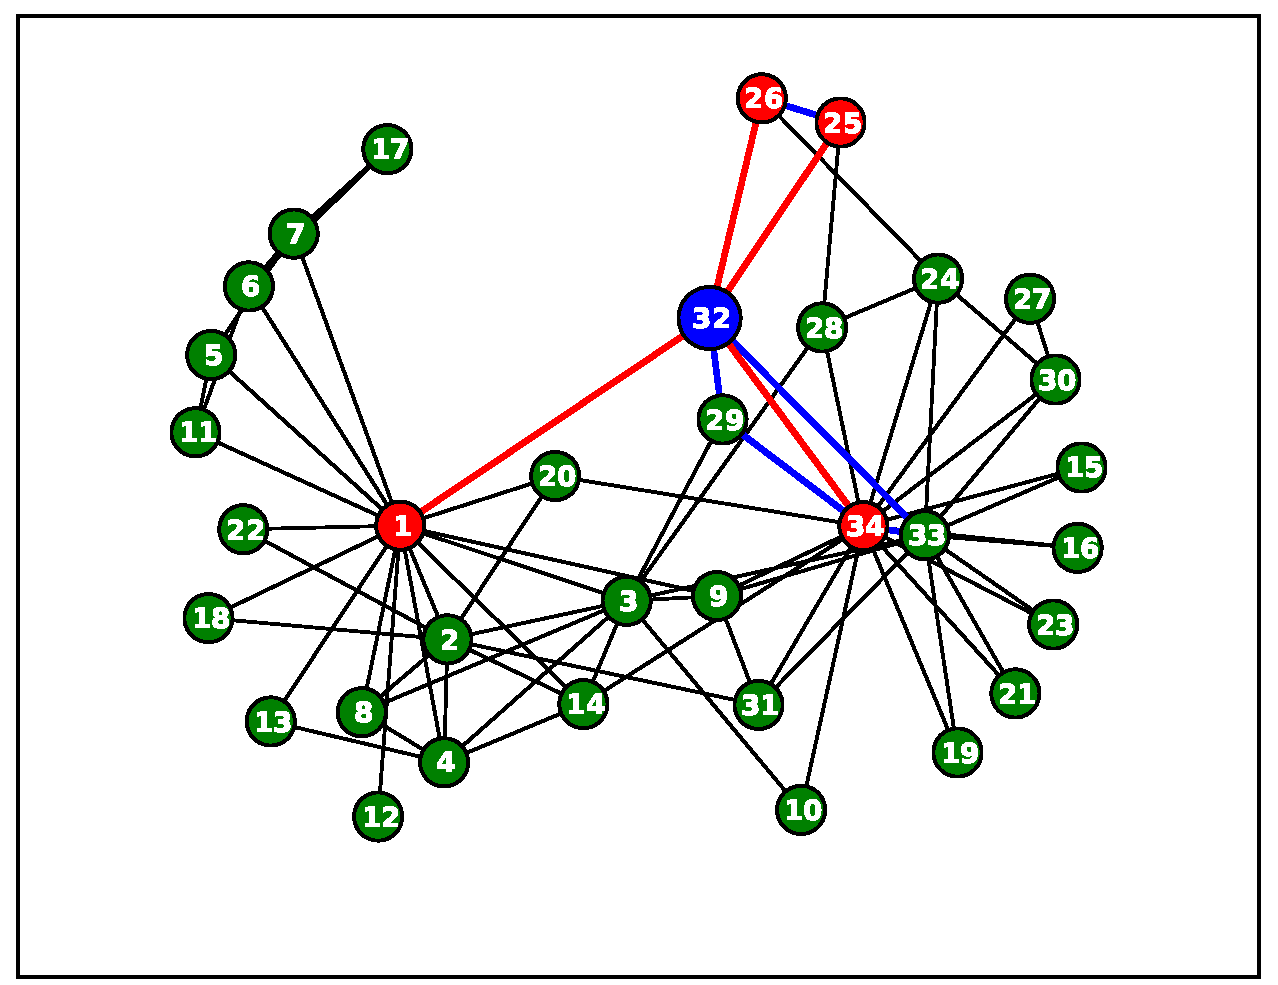
\includegraphics[scale=0.36]{./chap5/SD2}}
	
	\caption{以Zachary俱乐部网络为例,节点32,接受不同圈子信息的多样性结构}
	\label{fig:chap05egonetwork}
\end{figure}
我们以节点[32]作为信息的接收点,如图~\ref{fig:chap05SD2}所示,假设你同时从你研究生同学节点[25,26]分别得到一信息,其可信度与你分别从高中同学[1]和大学同学[34]得到一消息是完全不同的,你对后一种情况下信息的可信性和感兴趣程度将倍增,你转发传播该信息的概率将会累积增加,参考了文献\cite{ugander2012structural}。

从信息接收者的角度来看,其是否会推动信息的传播由其自身的内部因素决定的同时,也与其所处的外部环境密切相关。我们所提出的信息传播模型同时也考虑了这两方面的因素。我们根据传播信息节点与未知信息节点关系紧密程度,及信息传播结构的多样性,从以下几个方面对进行了分析、考虑和划分,并给出了实验分析结果及比较。
\begin{enumerate}[(1)]
	\item 从重叠社区划分角度分析,每个节点可以属于多个社区(团体)。重点参考、分析了Clique划分方法\cite{palla2005uncovering}。
	\item 对重叠社区的Clique方法限制进行了放宽,从K-trussess角度分析\cite{cohen2008trusses,csermely2013structure,redmond2012mining,huang2014querying,rossi2014fast}。
	\item 从无重叠社区划分(Community)\cite{newman2004finding}角度分析,每个节点只属于唯一的一个社区。因为不同的算法划分社区的模块优化值不同,社区节点之间的紧密程度也不尽相同。
	\item 从连通子图角度分析,每个一节点所属的Ego网络如果节点的邻居节点之没有连通,我们就认为他们属于不同的社区(或圈子)。
\end{enumerate}

%同时我们的模型也可成为重要热点人物发现,热点团体发现的研究基础。这为信息的研究提供了新的思路和方法。

\section{ISSD模型与算法}
\subsection{信息传播假设}
我们根据信息传播的特性做出以下假设:
\begin{assumption}
\label{chap5:assumption1}
	信息传播具有记忆性、累积性。
\end{assumption}

这与疾病传播是不同,个体在没完全接受之前,信息会留在记忆中,只是会因为对信息的兴趣程度,所留下的印象程度有所不同。

\begin{assumption}
\label{chap5:assumption2}
	信息传播具有活性。%人们接受心理不同
\end{assumption}

信息活跃程度会随外界、周围信息环境变化,会随时间快速增加然后迅速衰减。A.M.Treisman\cite{treisman1980feature}的过虑器理论模型认为,在多通道信息加工过程中,信息得到处理的程度不同,某些信息通过过滤器时会被衰减,实验证明衰减模型能对人的行为做出很好的预测。

\begin{assumption}
\label{chap5:assumption3}
	信息传播具有社会加强性。%信息的累积性,及多样性的增强效应
\end{assumption}

特别是由于所处的环境具有结构多样性,其加强性表现的更加突出。譬如当你高中圈子的一个同学说一信息时你可能没太在意,可是高中同学圈子越来越多的同学说该信息,你开始留意了;但是你大学同学的圈子也在讨论这一件事,那么你这个信息的可信性和感兴趣程度将倍增,你相信该信息的概率将会累积增加。

\begin{assumption}
	\label{chap5:assumption4}
	信息接受程度不同。%连权重
\end{assumption}

信息传播中由于网络成员之间关系不同,对不同联系人员所传播信息内容信任程度和接受程度不同。如在我们现实生活朋友圈子中,我们对铁哥们(闺蜜),亲密朋友及认识朋友传来的信息信任程度是完全不同的。
\begin{assumption}
	\label{chap5:assumption5}
	信息传播中传播个体存在差异。
\end{assumption}

信息传播中不同传播者,由于每个个体自身年龄、文化程度、知识背景、工作性质、生活环境等不同,对信息内容的兴趣程度不同存在差异。%个体阈值不同
\subsection{信息传播机理}
结合相关研究,我们把社会网络中个体(节点)对信息的了解程度分为未知信息状态(\underline{\textbf{U}}nknown),表示没有接收到信息;得知信息状态(\underline{\textbf{K}}nown),接收到信息但是不准备传播信息;传播信息状态(\underline{\textbf{A}}pproved),发送信息、传播信息;信息疲惫态(\underline{\textbf{E}}xhausted),不再传播已传播的信息,只是接收但是放弃传播信息等四种状态类型。社会网络中,一个用户产生或发布一条信息会传播到与其连接的邻居用户,然后自己在下一个时间阶段对此信息失去兴趣,不再重复传播,变为信息疲惫者;邻居用户得知这条信息后根据个人的喜好、兴趣程度等因素或者成为得知信息状态或者成为传播信息状态,若得知信息状态用户受信息累积而传播此信息,即其信息状态由得知信息状态变为传播信息状态;在信息传播过程中如果遇到信息疲惫状态用户,信息将不被传播。传播过程个体用户状态转变过程如图~\ref{fig:SDIMgraph}所示。
\begin{figure}[H] % use float package if you want it here
	\centering
	\includegraphics[scale=0.7]{./chap5/SDIMgraph}
	\caption{信息传播节点状态转变示意图}
	\label{fig:SDIMgraph}
\end{figure}

%信息在U、K、A、E四种状态之间的传播规则描述如下:
%\begin{enumerate}[(1)]
%\item 对于确认信息节点会以$p_1$的概率影响其邻居节点,使其邻居节点转变为,$p_1$的值为节点之间的影响力、所处网络结构等因素量化所得。
%\item 对于确认信息节点会以$p_1$的概率影响其邻居节点,使其邻居节点转变为
%\end{enumerate}

我们以著名的Zachary\cite{zachary1977information}空手道俱乐部成员关系网络为例(如图~\ref{fig:ZacharyS1}所示),给出信息传播过程中每个节点的信息状态随时间的演变过程,设定初始传播信息节点为[1,34],如图~\ref{fig:chap05ZacharySpreading}所示。
\begin{figure}[H] % use float package if you want it here
	\centering
	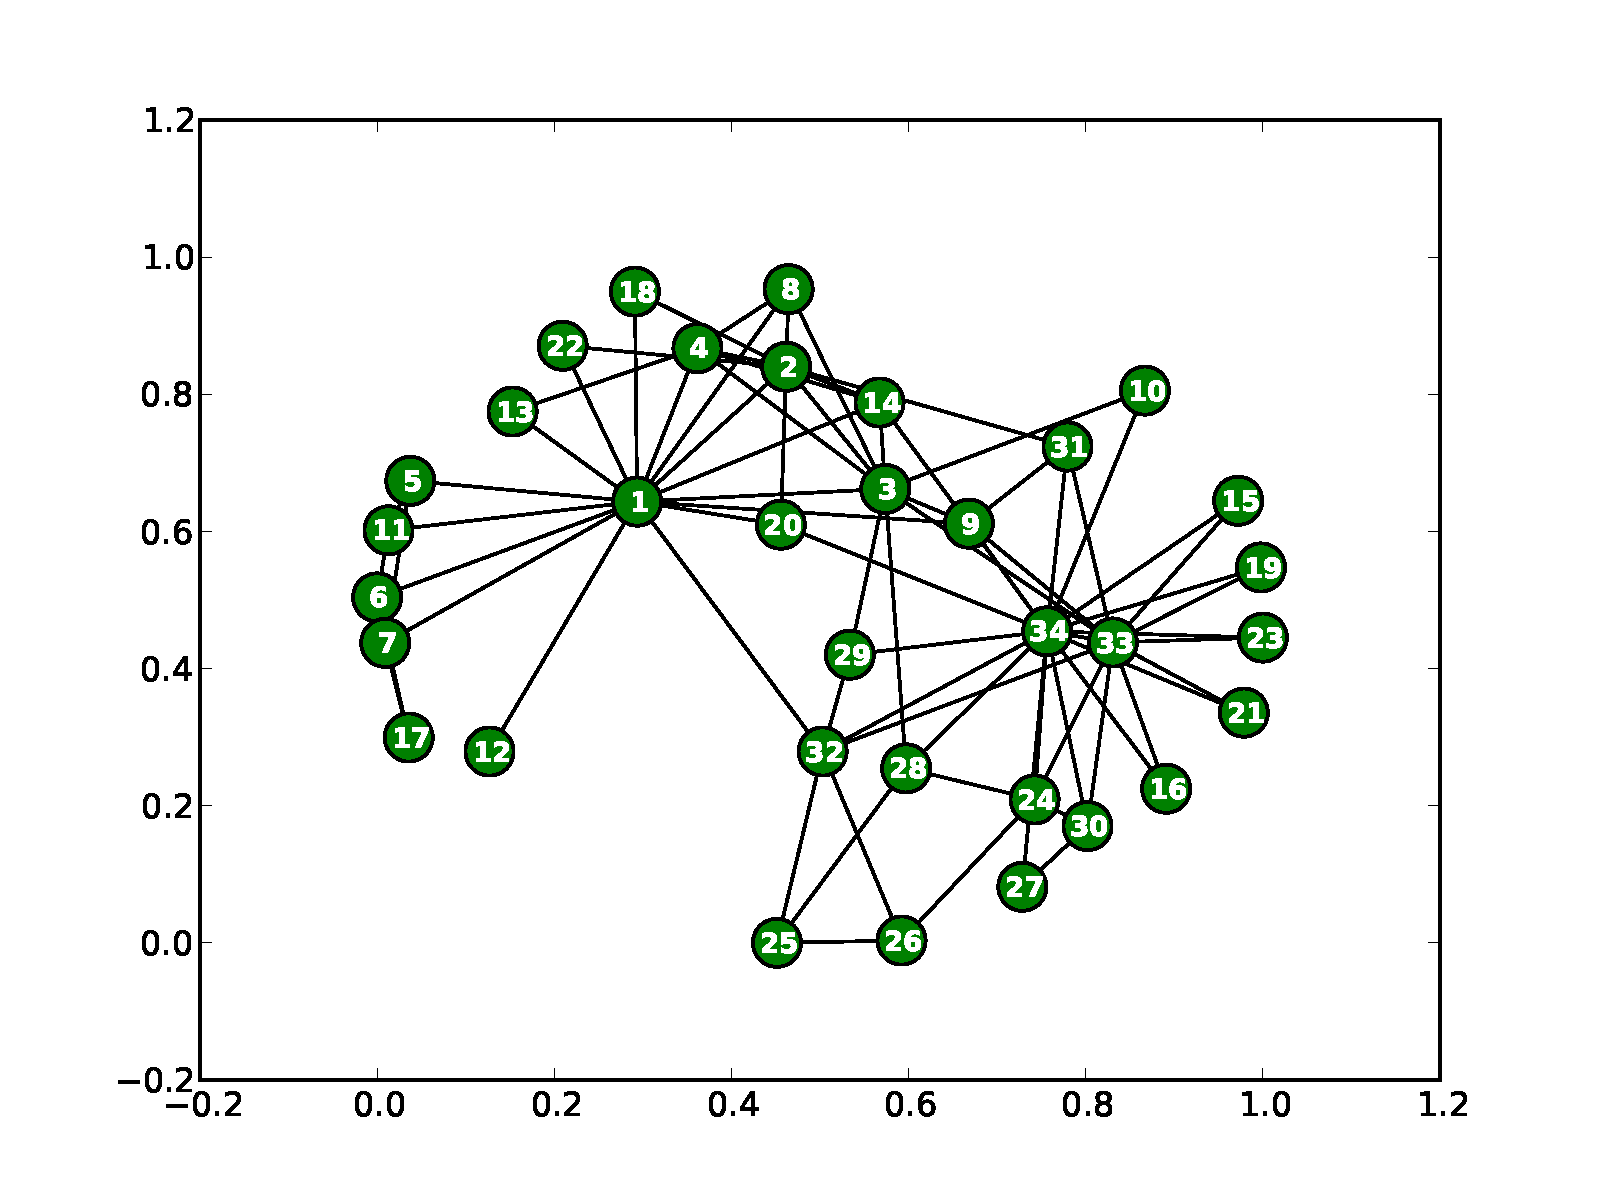
\includegraphics[scale=0.8]{./chap5/ZacharyS1}
	\caption{Zachary 俱乐部人员网络关系图}
	\label{fig:ZacharyS1}
\end{figure}
%ISSDgraph
\begin{figure}[H]
\centering%
	\subcaptionbox{t=1\label{fig:ZacharyS2}}
	%标题的长度,超过则会换行,如下一个小图。
	{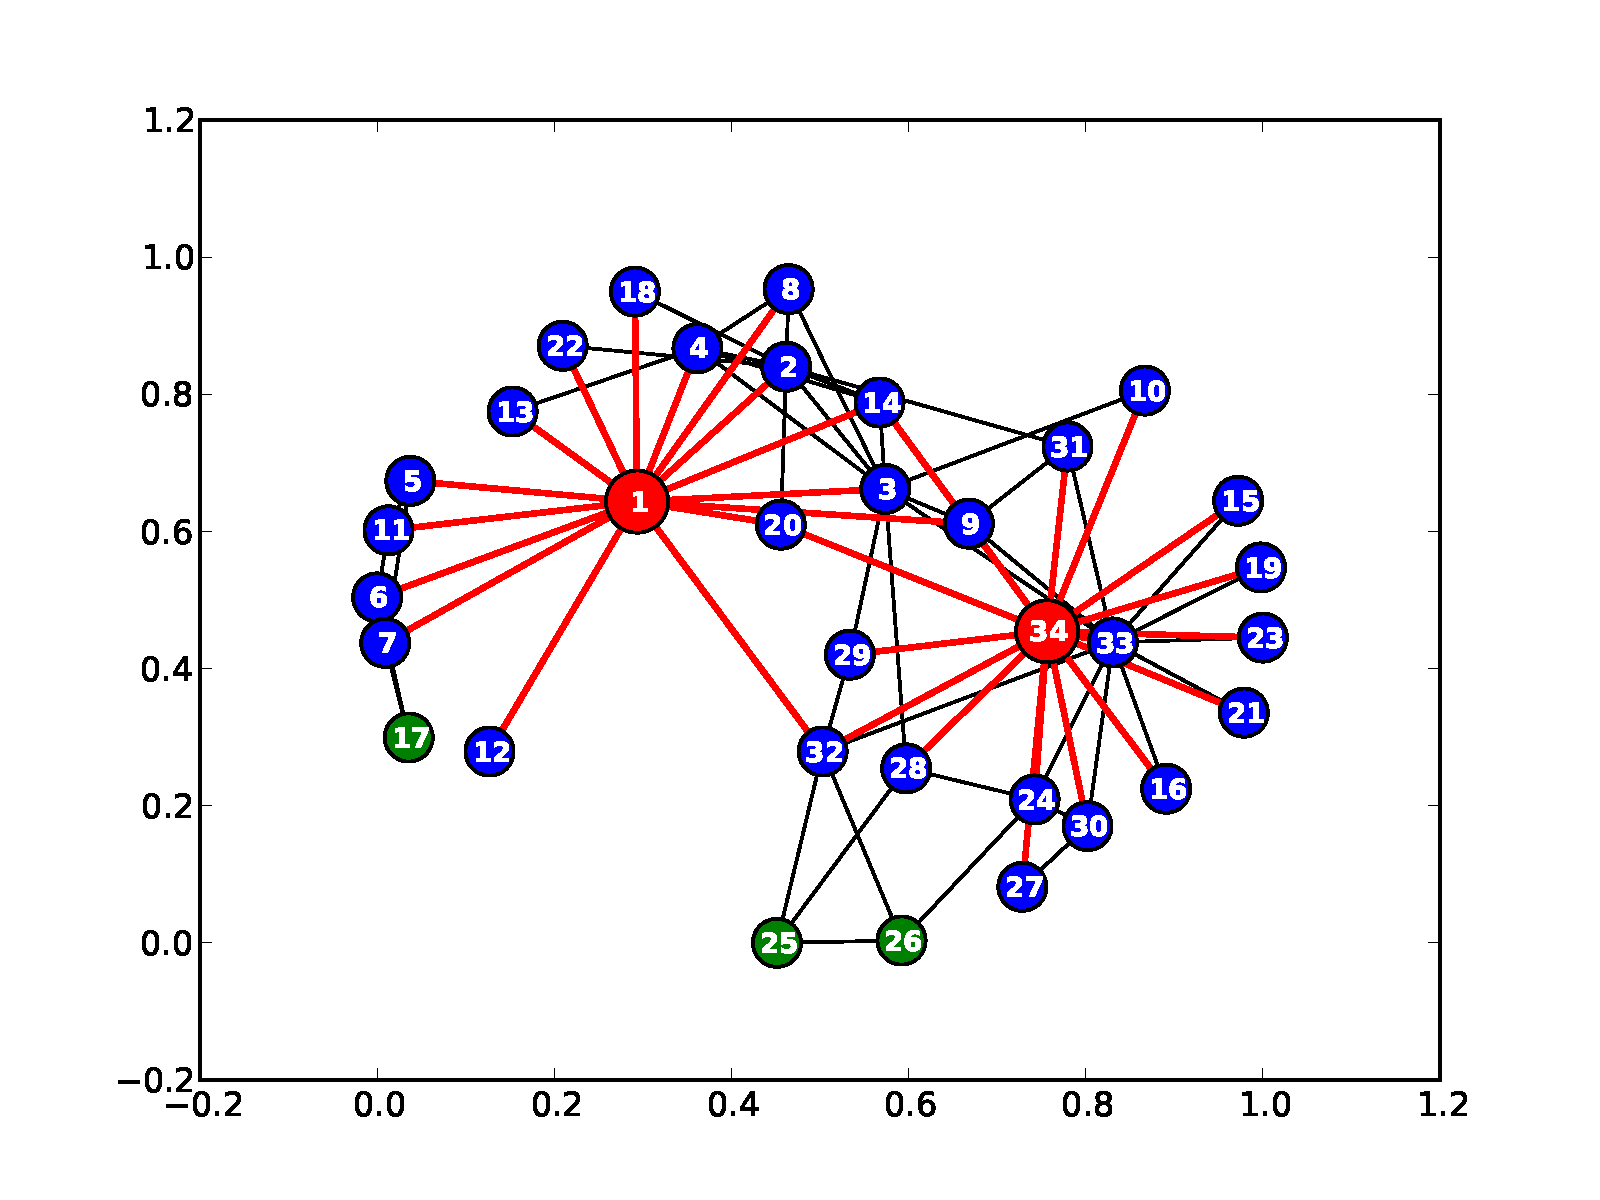
\includegraphics[scale=0.36]{./chap5/ZacharyS2}}
	\hspace{1mm}%
	\subcaptionbox{t=2\label{fig:ZacharyS3}}
	{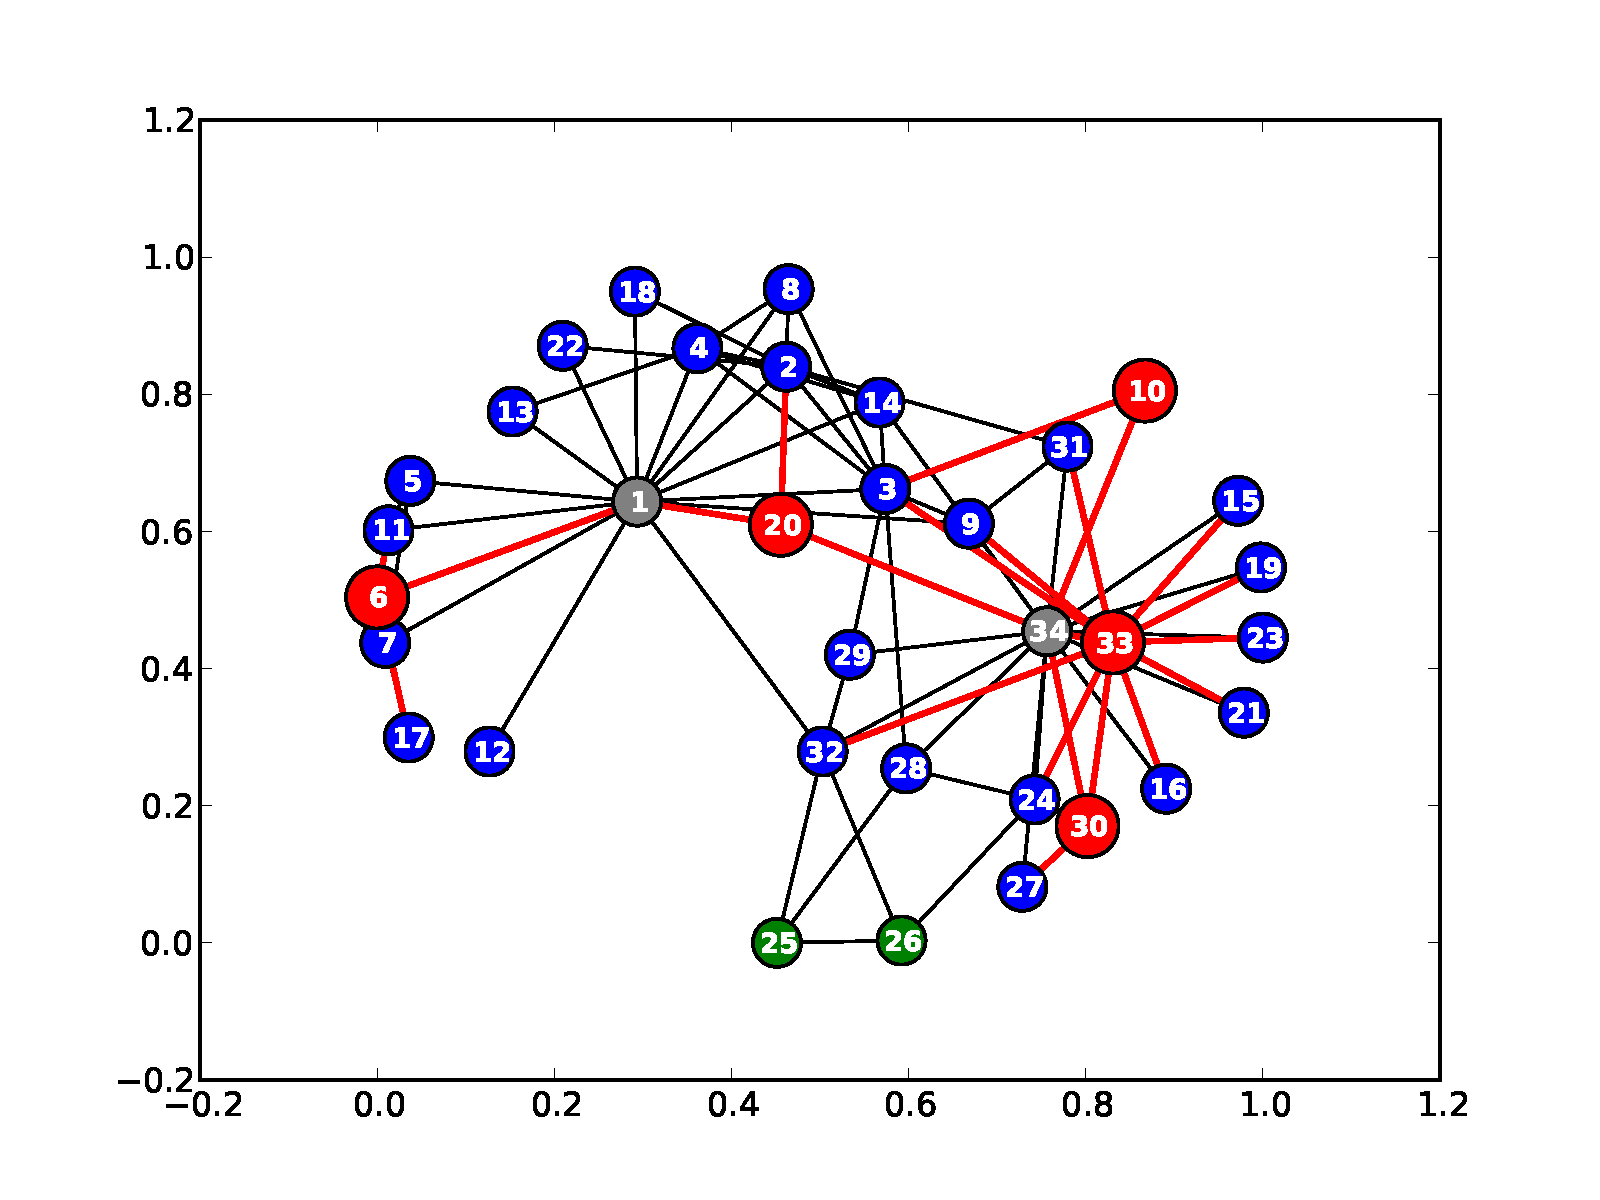
\includegraphics[scale=0.36]{./chap5/ZacharyS3}}
	
	\subcaptionbox{t=3\label{fig:ZacharyS4}}
	%标题的长度,超过则会换行,如下一个小图。
	{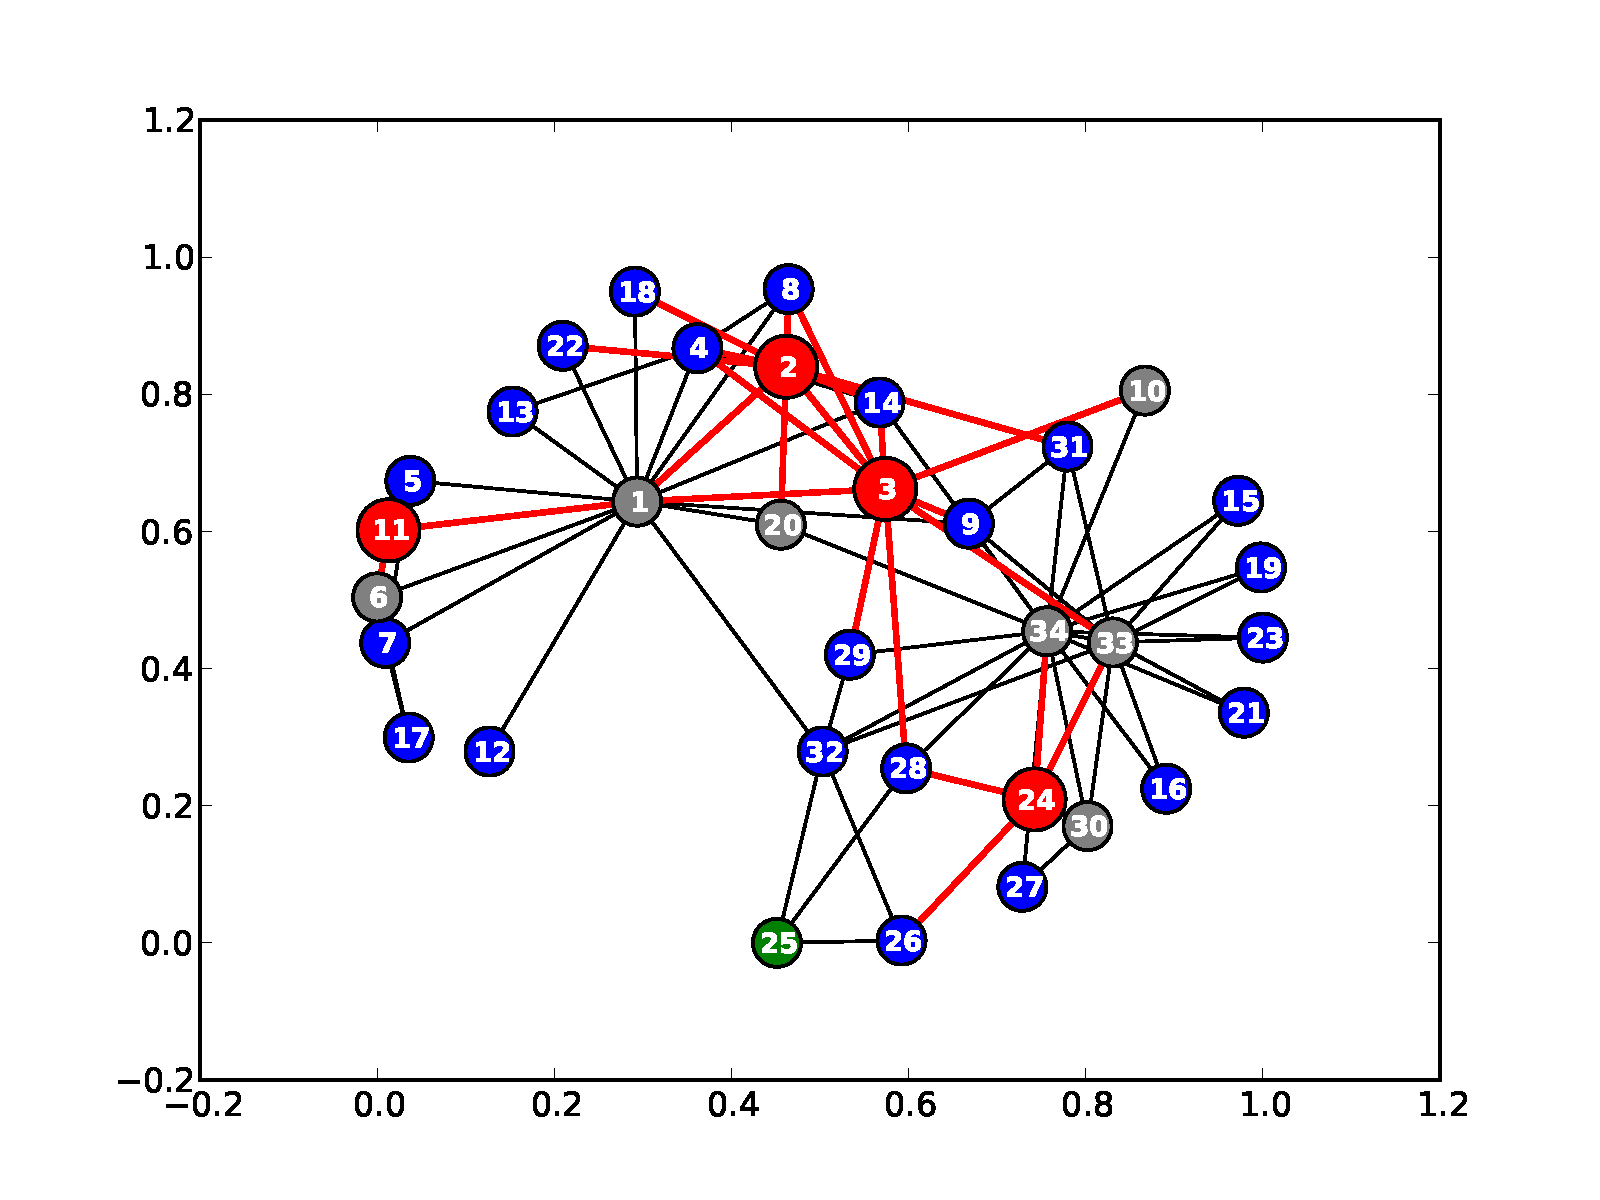
\includegraphics[scale=0.36]{./chap5/ZacharyS4}}
	%\hspace{3em}%
	\subcaptionbox{t=4\label{fig:ZacharyS5}}
	{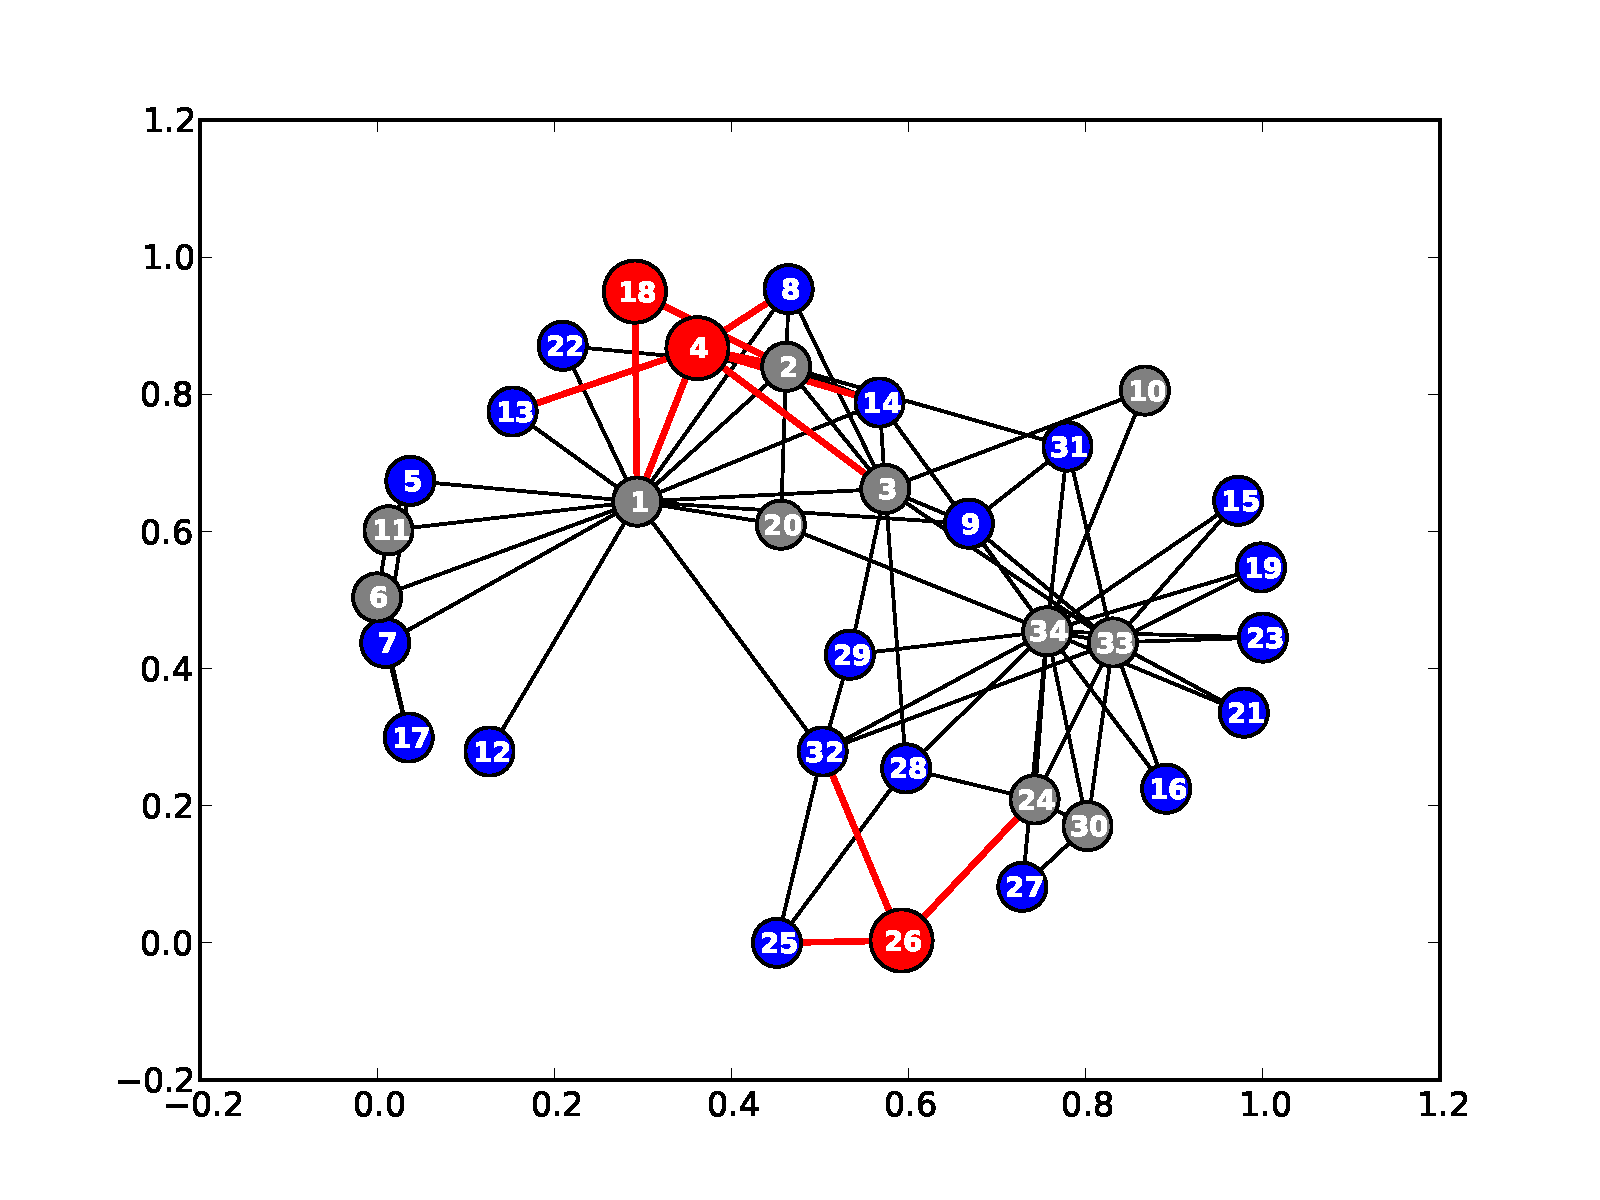
\includegraphics[scale=0.36]{./chap5/ZacharyS5}}
	
	\subcaptionbox{t=5\label{fig:ZacharyS6}}
	%标题的长度,超过则会换行,如下一个小图。
	{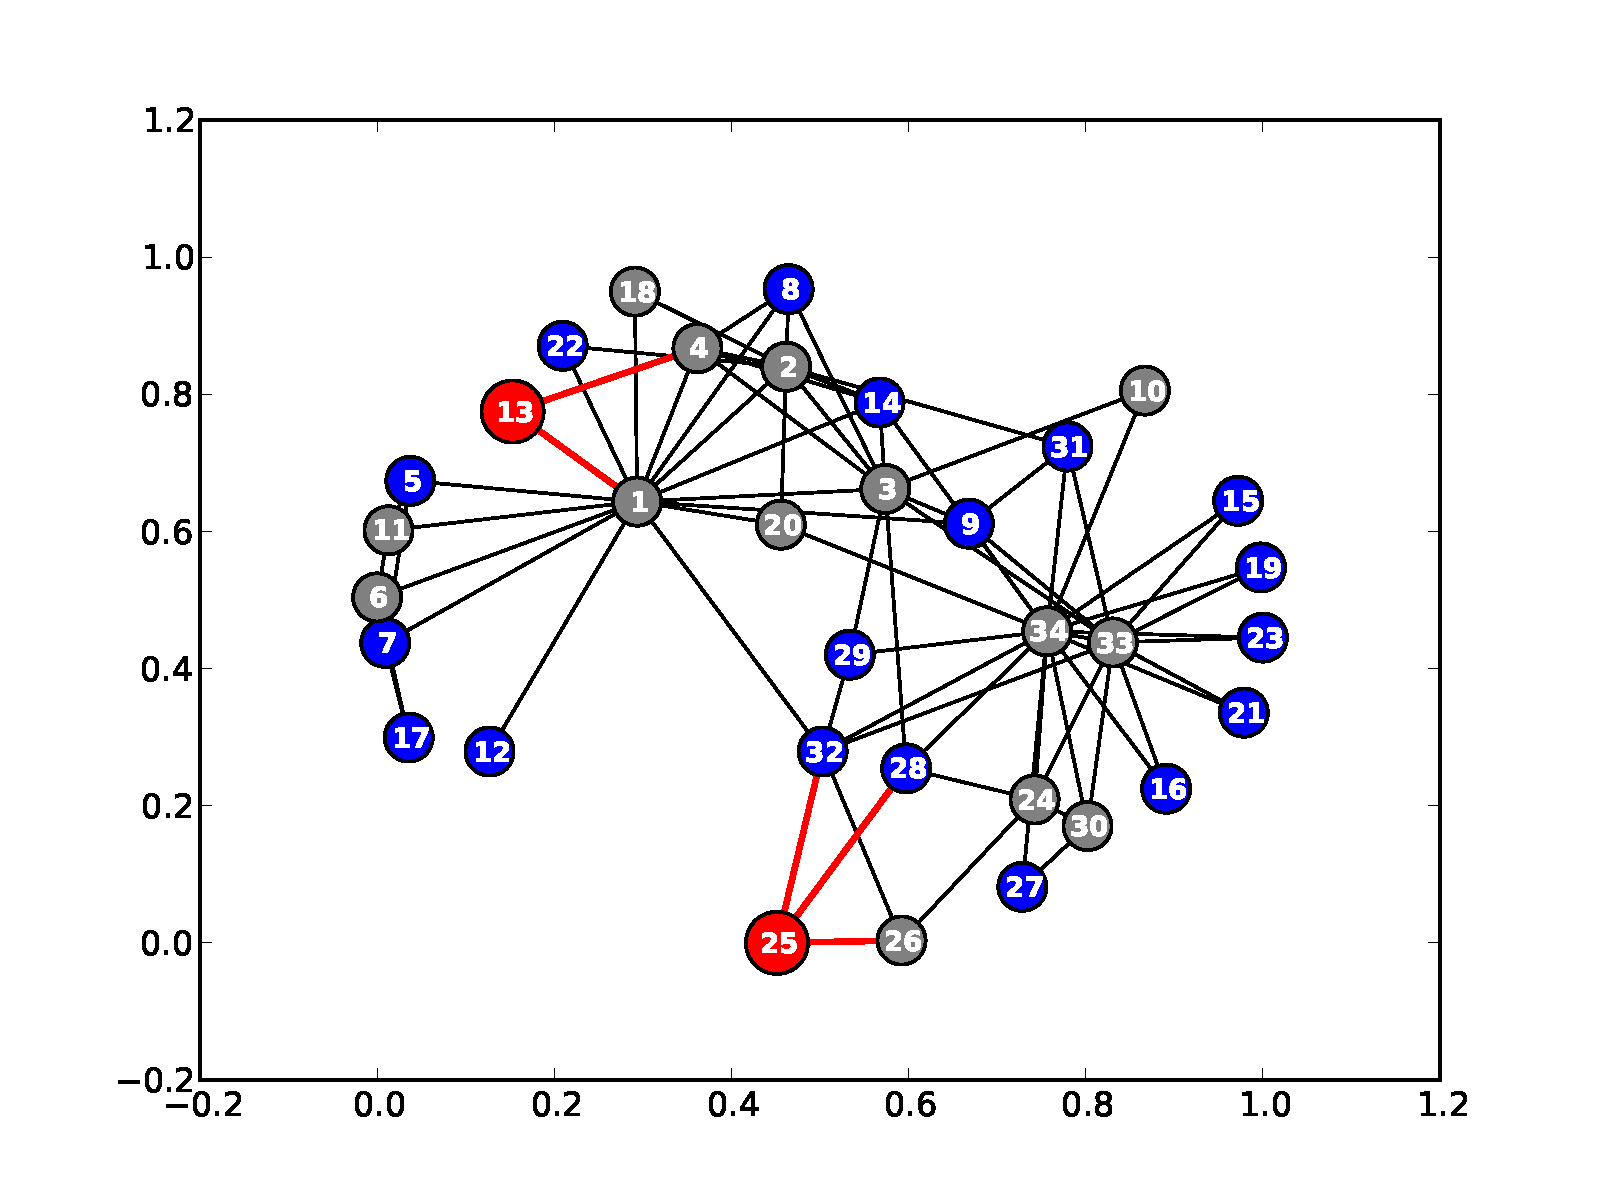
\includegraphics[scale=0.36]{./chap5/ZacharyS6}}
	%\hspace{2em}%
	\subcaptionbox{t=6\label{fig:ZacharyS7}}
	{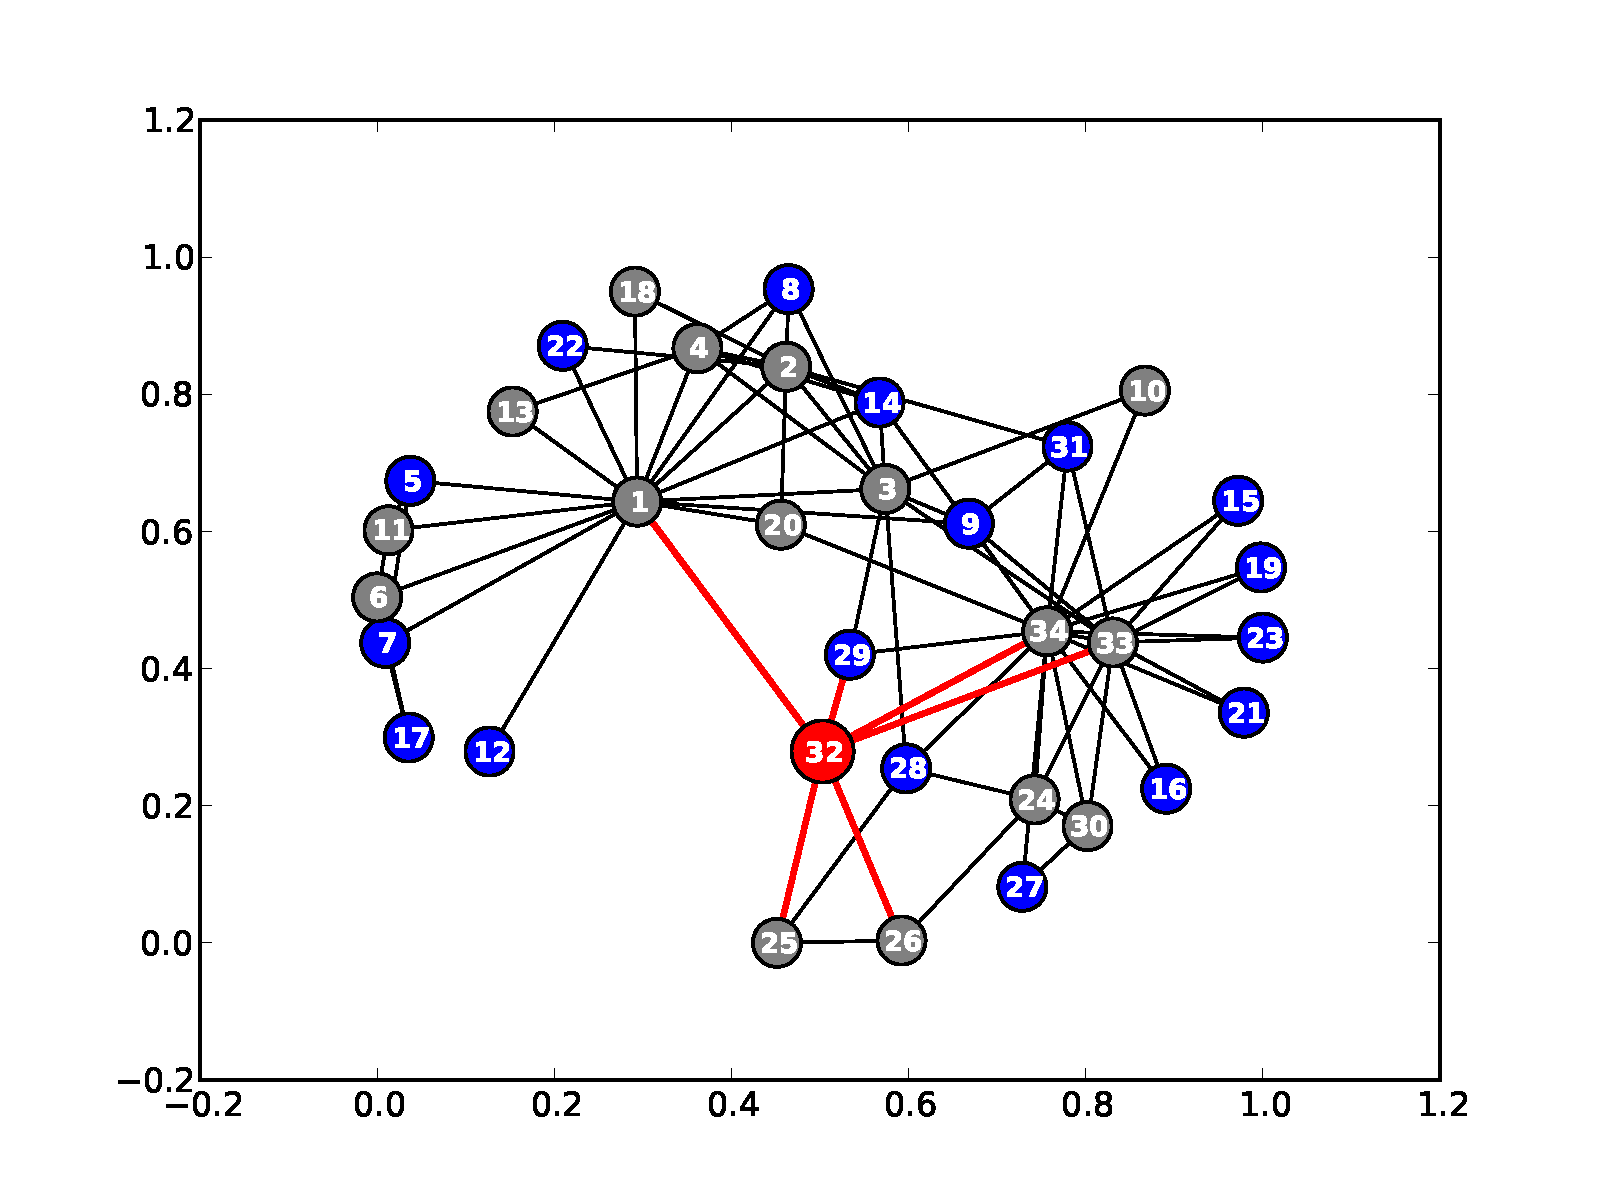
\includegraphics[scale=0.36]{./chap5/ZacharyS7}}
	\caption{以Zachary网络为例,选定初始信息传播种子节点为[1、34],随着时间信息传播演化过程}
	\label{fig:chap05ZacharySpreading}
\end{figure}

%\section{ISSD模型与算法}

\subsection{基本概念定义}
信息传播的社会网络可以描述为由节点及节点之间的边组成的复杂网络结构,$G(V,E,A)$,其中$V$是所有结节的集合,节点的个数为$n=|V|$,节点的属性可以是个体自身特征,如用户的爱好、所属社区、年龄、性别等。$E$为所有边的集合,为$E\subseteq V\times V$,$e_{uv}\in E$且$(u,v \in V)$,边的个数为$m=|E|$,边的属可以为节点之间的影响权重、紧密程度等。$A$为图的属性,可以是图的名称代号、网络结构特点等。无重叠社区划分(Community)$(c_1,c_2,\dots,c_n|c_i \in C)$,且$c_i\cap c_j = \phi$。有重叠社区划分(K-clique)$(k_1,k_2,\dots,k_n|k_i \in K)$,且$|k_i\cap k_j| \geq 0$。 有重叠社区划分(K-trusses)$(tr_1,tr_2,\dots,tr_n|tr_i \in Tr)$,且$|tr_i\cap tr_j| \geq 0$。网络连通子图(Connected Component)$(cc_1,cc_2\dots,cc_n|cc_i \in Cc)$,且$|cc_i\cap cc_j| \geq 0$。

信息随时间传播过程行为形式化描述为:$I(V,E,T)$,某个信息$(i_1,\dots,i_n|i_j \in I)$,传播时间$(t_1,t_2,\dots,t_n|t_i \in T)$。例如$i_j(u,t_1)$,表示为节点$u$在时间$t_1$产生了信息$i_j$。$i_j(e_{uv},t_2)$,表示为节点$u$在$t_2$时间将信息$i_j$传播给了邻居节点$v$,具体过程如图~\ref{fig:chap05VETgraph}所示。
\begin{figure}[H] 
	\centering
	\includegraphics[scale=1.0]{./chap5/chap05VETgraph}
	\caption{信息随时间传播过程形式化描述样例}
	\label{fig:chap05VETgraph}
\end{figure}
\subsection{ISSD模型}
信息传播过程具有复杂多样性,及不确定性。这里我们重点考虑信息传播过程所具有的5个假设特性,提出了信息传播结构多样性模型(ISSD,Infomation Spreading Structural Diversity Model)。
以前研究模型和方法主要从传播节点触发、激活其它节点的角度分析问题,而我们从被触发或将要被激活的节点这一独特的角度分析和解决问题。我们认为未知信息节点(\textbf{U})被激活(或感染)的概率不但与传播信息节点(\textbf{A})之间的关系程度有关,即在网络关系图中表示 为节点之间边的权重。我们还特别考虑了接收信息节点所处的外部环境这个外部因素,如其所在的社区结构多样性特征等;同时我们也着重考虑了信息传播时间变化因素。总体与哲学范畴中“事物的发展是内因、外因共同起作用的结果”思想相符。这也与第~\ref{cha:3thChap03}章节中最具影响力节点发现思路也是一致的。

ISSD模型可以描述为
:在复杂网络$G=(V,E,A)$中,定义$N(u)$为节点$u$的邻居节点集合,$X$为某种社区划分方法,$(x_1,\dots,x_n|x_i \in X)$,$X$可以为社区划分中的C、K、Tr、Cc等。未被激活(未知信息)的节点$u$,不但受其激活邻居节点$S_a$(传播信息节点)中$v$所产生的影响力$b_{uv}$影响,同时受其Ego网络中激活邻居节点所在的结构多样性变化的社区环境影响,参阅假设,如信息传播的社会加强性,信息在“影响积累”的同时也会随周围信息的冷热度进行变化,但是一个节点$u$的受其所有激活邻居节点对$u$的影响力总和小于等于1,即:
\begin{equation} 
{\sum_{x_i=1}^{x_i=k}   {\sum_{v \in N(u),v\in S_a}} b_{uv} \leq 1} 
\end{equation}
我们假设每个节点$u$有一个激活特定阈值$\theta_u\in\left[0,1\right]$,如果${\sum_{x_i=1}^{x_i=k}   {\sum_{v \in N(u),v\in S_a}} b_{uv} \geq \theta_u}$,则节点$u$由未知状态(U)被激活为传播信息状态(A)。在ISSD模型中,当某个圈子(或社区)的一个激活节点$v$尝试激活它的未激活邻居$u$没有成功时,那么节点$v$对节点$u$的影响力被积累起来,信息从不同圈子来,可信度、影响力是不同的,这样对后面其它已激活的邻居节点对$u$的激活是有贡献的。直到所有节点被激活或没有新的节点再被激活,信息传播的整个过程结束。这就是ISSD模型中信息传播结构多样性的特性,这与IC模型、LT模型及传染病模型等所不同的。

下面我们加入信息传播时间变化因素。具有时间特征的ISSD模型可描述为,每个节点$u$都有确认传播信息的阈值$\theta_u \in [0,1]$。对于节点$u$会受其邻居中已传播信息状态(也叫激活状态)节点$v\in N(u), v\in S_a$的影响,设其中$g(u,t)$为节点$u$在时间$t$时,受其邻居节点中确认信息状态节点的结构多样化影响程度函数;$f(u,t)$为节点$u$在时间$t$时的信息累积程度函数。且${\sum_{x_i=1}^{x_i=k}   {\sum_{v \in N(u),v\in S_a}} b_{uv} \le \theta_u}$,其中$X \subseteq ({C\cup K\cup Tr\cup Cc}) $。那么在$t + 1$时,当满足条件:
\begin{equation}
\label{chap05infocoolsumtheta}
\begin{split}
& f(u,t_1){\sum_{v \in N(u),v\in S_a}} g(u,t_1)b_{uv} + f(u,t_2){\sum_{v \in N(u),v\in S_a}} g(u,t_2)b_{uv} + \cdots \\
& + f(u,t_{t+1}){\sum_{v \in N(u),v\in S_a}} g(u,t_{t+1})b_{uv}  \geq \theta _u
\end{split}
\end{equation}
时,节点$u$将变为激活状态。模型中参数在不同类型的信息传播网络中是不同的,节点对不同种类的信息传播初始阈值也不相同,参数的变化可以根据实际情况来确定。下面给出了模型的相应算法。

\subsection{ISSD算法}
为了对ISSD算法表述方便,表~\ref{tab:ISSD_table}列出了相关重要变量参数。
\begin{table}[htbp]
	\centering
	\begin{minipage}[t]{0.9\linewidth}
		\caption{ISSD算法参数描述说明}
		\label{tab:ISSD_table}
		%\begin{tabular}{*{7}{p{.14\textwidth}}}
		\begin{tabular}{p{2.1cm}p{9cm}}
			\toprule[1.5pt]
			\heiti 变量 &  \heiti 说明描述 \\  
			\midrule[1pt]
			$S$& 初始传播的种子节点 \\
			$S_a$& 传播信息状态的节点 \\
			$S_k$& 得知信息状态的节点,对信息进行了累积记忆 \\
			$S_e$& 信息疲惫状态的节点,节点不再传播已传播的信息 \\
			$newS_a$& 新的被激活传播信息状态的节点 \\
			$time$& 信息传播的时间 \\
			$neighbor(u)$& 与节点$u$连接的邻居节点 \\
			$x$& 节点归属哪个社区,可以为无重叠社区(Community)、重叠社区(K-clique)、连通子图和K-trusses子图等社区划分结果 \\
			$f(x,t)$& 信息传播随时间变化的衰减(增强)函数 \\
			$g(x,t)$& 信息传播结构多样性函数 \\
			\bottomrule[1.5pt]
		\end{tabular}
	\end{minipage}
\end{table}

信息传播结构多样化传播算法描述如算法4所示:
\begin{algorithm}
	\caption{ISSD(G,S)}%Infomation Spreading Structural Diversity Model
	\label{alg:chap5:ISSDalgorithm}
	\begin{algorithmic}[1]
		\STATE $S_a=newS_a=S; S_e \leftarrow \Phi; S_k \leftarrow \Phi; time = 1$
		\WHILE {$|S|\geq 0$}
		\STATE $S_k = neighbor(S)$;$newS_a \leftarrow \Phi$
		\FOR {each  vertex $v \in S_k\setminus S$ }
		\FOR {each vertex $u \in S $}
		\IF {$\sum_{v \in x}(f(g(x,t),t)e_{uv}[weight]) \geq \theta_u$ }
		\STATE $newS_a = newS_a \cup \{v\}$
		\ENDIF
		\ENDFOR
		\ENDFOR
		\STATE time +=  1
		\STATE $S_e = S_e \cup S_a $;$S_a = S_a \cup newS_a$;$S_k=S_k \cup \setminus S$
		\STATE $S=newS_a$;
		\ENDWHILE
		\RETURN $S_e,S_a,S_k$
	\end{algorithmic}
\end{algorithm}

\section{实验结果与分析}
\subsection{ISSD时间影响}
我们通过在实际关系网络实验分析,发现了信息传播过程与我们以往认知不同的现象,一般认为,度数大的个体节点是推动信息传播的主要因素和关键因素,初始传播源节点集合的影响力越多,传播范围越大。但我们对节点按度数大小进行排序,逐步增大度数Top-k初始传播节点集合,由于某些节点的加入时机不同,反而阻碍了信息的传播,使传播范围反而明显减小。

这里以《悲惨世界》人物关系网络\cite{knuth1993stanford}为例进行说明。如图~\ref{fig:chap05lesmis}所示,数据源\cite{knuth1993stanford}是D. E. Knuth 整理了小说的人物关系网络,节点表示小说中的角色,边表示两个角色同时出现在一幕或多幕中,网络关系如图~\ref{fig:chap050lesmis}所示。
\begin{figure}[H] 
	\centering
	\includegraphics[scale=0.6]{./chap5/0lesmis}
	\caption{悲惨世界人物关系网络节点表示}
	\label{fig:chap050lesmis}
\end{figure}

网络中主要人物如表~\ref{tab:lesmisNodeMap}所示。
\begin{table}[!htb]
	\begin{minipage}[t]{1\linewidth}
		\centering
		\caption{悲惨世界人物关系网络中节点度数前10名}
		\label{tab:lesmisNodeMap}
		\begin{tabular}{p{.2\textwidth}<{\centering}p{0.2\textwidth}<{\centering}p{0.2\textwidth}<{\centering}p{0.1\textwidth}<{\centering}p{0.1\textwidth}<{\centering}}
			\toprule[1.5pt]
			{\heiti 人物英文名} & {\heiti 人物中文名} & {\heiti 角色} & {\heiti 编号} & {\heiti 度数} \\\midrule[1pt]
			Jean Valjean & 冉阿让 & 主人公 & 11 & 36 \\ 
			Gavroche & 加夫罗契 & 革命青年 & 48 & 22 \\ 
			Marius & 马吕斯 & 爱潘妮的弟弟 & 55 & 19 \\ 
			Javert & 贾维 & 探长 & 27 & 17 \\ 
			Thenardier & 德纳 & 酒馆的老板 & 25 & 16 \\ 
			Fantine & 芳汀 & 女工 & 23 & 15 \\ 
			Enjolras & 恩佐拉 & 革命青年 & 58 & 15 \\ 
			Courfeyrac & 古费拉克 & 学生 & 62 & 13 \\ %学生酱油党里稍微出挑一点的是Courfeyrac
			Bossuet & 博须埃 & 主教 & 64 & 13 \\ 
			Bahorel & 巴阿雷 & 学生 & 63 & 13 \\
			\bottomrule[1.5pt]
		\end{tabular}
	\end{minipage}
\end{table}
%\begin{table}[htb]
%	\centering
%	\caption{悲惨世界人物关系网络中节点度数前10名}
%	%\label{ISSD_table}
%	\label{tab:lesmisNodeMap}
%	\begin{tabular}{|c|c|c|c|c|} \hline
%		\heiti 人物英文名 & \heiti 人物中文名 & \heiti 角色 &  \heiti 编号 &  \heiti 度数 \\ \hline
%		Jean Valjean & 冉阿让 & 主人公 & 11 & 36 \\ \hline
%		Gavroche & 加夫罗契 & 革命青年 & 48 & 22 \\ \hline
%		Marius & 马吕斯 & 爱潘妮的弟弟 & 55 & 19 \\ \hline
%		Javert & 贾维 & 探长 & 27 & 17 \\ \hline
%		Thenardier & 德纳 & 酒馆的老板 & 25 & 16 \\ \hline
%		Fantine & 芳汀 & 女工 & 23 & 15 \\ \hline
%		Enjolras & 恩佐拉 & 革命青年 & 58 & 15 \\ \hline
%		Courfeyrac & 古费拉克 & 学生 & 62 & 13 \\ \hline%学生酱油党里稍微出挑一点的是Courfeyrac
%		Bossuet & 博须埃 & 主教 & 64 & 13 \\ \hline
%		Bahorel & 巴阿雷 & 学生 & 63 & 13 \\ \hline
%	\end{tabular}
%\end{table}

为了保证实验现象的普遍性,我们对悲惨世界网络中节点随机设定在[0,1]之间初始阈值,且整体初值设定整体符合指数正态分布\cite{limpert2001log,holgate1989lognormal}。对于节点之间的相互影响力随机设定,且满足在[0,1]的正态分布\cite{lodzimierz1995normal,patel1996handbook,amari2007methods}。我们选择度数最大的节点[11],作为初始传播源节点,随着时间各节点信息状态的演化结果,如图~\ref{fig:chap05node1lesmis}。具体传播演化过程为: \\
$  t=1,[11] \rightarrow t=2,[10, 15, 27] \rightarrow t=3,[70, 29, 24] \\ 
\rightarrow t=4,[68, 69, 23, 25, 58] \rightarrow t=5,[21, 41, 57, 65, 71, 75] \\ 
\rightarrow t=6,[16, 17, 19, 48, 55, 59, 62, 63, 76] \rightarrow t=7,[18, 20, 22, 60, 61, 64, 66]$

\begin{figure}[H]
	\centering%
	\subcaptionbox{t=1\label{fig:chap0511lesmis}}
	%标题的长度,超过则会换行,如下一个小图。
	{\includegraphics[width=7.3cm]{./chap5/11lesmis}}
	%\hspace{3em}%
	\subcaptionbox{t=2\label{fig:chap0512lesmis}}
	{\includegraphics[width=7.3cm]{./chap5/12lesmis}}

\end{figure}
\addtocounter{figure}{-1}       %先欺骗LaTeX图形计数器
\begin{figure}[H]
	\addtocounter{figure}{1}
	\centering%
	\subcaptionbox{t=3\label{fig:chap0513lesmis}}
	{\includegraphics[width=7.3cm]{./chap5/13lesmis}}
	%\hspace{3em}%
	\subcaptionbox{t=4\label{fig:chap0514lesmis}}
	{\includegraphics[width=7.3cm]{./chap5/14lesmis}}
	\subcaptionbox{t=5\label{fig:chap0515lesmis}}
	%标题的长度,超过则会换行,如下一个小图。
	{\includegraphics[width=7.3cm]{./chap5/15lesmis}}
	%\hspace{3em}%
	\subcaptionbox{t=6\label{fig:chap0516lesmis}}
	{\includegraphics[width=7.3cm]{./chap5/16lesmis}}
	\subcaptionbox{t=7\label{fig:chap0517lesmis}}
	{\includegraphics[width=7.3cm]{./chap5/17lesmis}}
	\caption{节点11作为初始传播源节点传播过程}
	\label{fig:chap05node1lesmis}
\end{figure}
如图~\ref{fig:chap05node4lesmis}所示,我们选择连接度数最大的节点[11,48,55,27],作为初始传播源节点,随着时间各节点信息状态的演化结果。具体传播演化过程为: \\
$  t=1,[11, 48, 55, 27] \rightarrow t=2,[10, 15, 57, 65] \\
\rightarrow t=3,[58, 59, 63] \rightarrow t=4,[64, 66, 76, 60, 61, 62] 
$
\begin{figure}[H]
	
	\centering%
	\subcaptionbox{t=1\label{fig:chap0541lesmis}}
	{\includegraphics[width=7.3cm]{./chap5/41lesmis}}
	%\hspace{3em}%
	\subcaptionbox{t=2\label{fig:chap0542lesmis}}
	{\includegraphics[width=7.3cm]{./chap5/42lesmis}}
\end{figure}
\addtocounter{figure}{-1}       %先欺骗LaTeX图形计数器
\begin{figure}[H]
	\addtocounter{figure}{1}
	\centering%
	\subcaptionbox{t=3\label{fig:chap0543lesmis}}
	{\includegraphics[width=7.3cm]{./chap5/43lesmis}}
	%\hspace{3em}%
	\subcaptionbox{t=4\label{fig:chap0544lesmis}}
	{\includegraphics[width=7.3cm]{./chap5/44lesmis}}
	\caption{节点11,48,55,27作为初始传播源节点传播过程}
	\label{fig:chap05node4lesmis}
\end{figure}

从图~\ref{fig:chap05node4lesmis},图~\ref{fig:chap05node1lesmis}我们可以看到与传统思路相反的结果,即一般认为,越多的影响力节点加入,越能推动整个传播过程。以下我们分析了产生与传统想法相反现象的原因:
\begin{enumerate}[(1)]
	\item 一些关键节点过早地成为信息疲惫状态,中断了信息传播的持续加强性;
	\item 信息传播对邻居节点的信息累积没有影响其信息状态,其后随时间快速衰减;
\end{enumerate}

我们知道信息传播是个复杂的传播演变过程,只是简单地应用传统知识是无法解释信息传播的原理的。另一方面信息传播不但和参与传播的节点相关,而且和参与者加入信息传播的时机密切相关。这也为今后研究提出了新的思考角度与挑战。

\subsection{ISSD结构多样性影响}
目前研究信息传播大多从传播(或已感染)节点去触发、激活其它节点的角度分析问题,而本文我们从被传播或将被激活节点这一独特的角度分析和解决问题,重点分析了被传播节点的Ego环境结构多样化。

目前普遍认为社交网络中度数大,传播速度是最大的,以度中心化指标来衡量信息传播最大化。如新浪微博中利用大V用户(粉丝多的)作为市场营销的注入点,希望通过他们能产生口碑效应(Word of mouth),\cite{trusov2009effects,chevalier2006effect}最终能信息最大化传播。前面章节也发现利用度中心化作为影响力最大化传播方法也存在问题,如“富人俱乐部”现象。例如我们选择Netscience合著网络\cite{boccaletti2006complex}中节点度最大的前10、20个节点形成关系子图,从图~\ref{fig:chap05netscienceTopKDegree}中我们可以看到排名前10中的节点[20,23,26,41]是个K-clique\cite{palla2005uncovering}是4的全连通图,他们是一个研究组的成员,通常他们学术研究内容或范围应该相近。通常会认为,如果其一名学者知道某种理论或技术,其他人员一般也会知道的,所以选择他们其中的任何一个成员传播源节点比较合理。
\begin{figure}[H]
	\centering%
	\subcaptionbox{节点度排名前10的节点关系\label{fig:chap05netscienceTop10Degree}}
	%标题的长度,超过则会换行,如下一个小图。
	{\includegraphics[width=7.3cm]{./chap5/netscienceTop10Degree}}
	%\hspace{3em}%
	\subcaptionbox{节点度排名前20的节点关系\label{fig:chap05netscienceTop20Degree}}
	{\includegraphics[width=7.3cm]{./chap5/netscienceTop20Degree}}
	\caption{合著网络中度排名Top-10(20)节点关系图}
	\label{fig:chap05netscienceTopKDegree}
\end{figure}
同时我们知道许多社会热点事件,大多不是由大V用户发起和主导的,在一定程度上这与他们参与热情及人们对他们信任程度等因素相关。我们知道,往往一些热衷于某些话题的草根用户,他们发起一些话题,然后爆发成为社会焦点或热点问题。

%Ego网络是整个上网络的子图,包括一个中心节点(ego)和其邻居节点,边包括中心节点与邻居节点,及其邻居节点之间的连线。如图~\ref{fig:chap05SD1}所示,以节点32中心的ego网络。
%
%\begin{figure}[H]
%	\centering%
%	\subcaptionbox{节点32的ego图\label{fig:chap05SD1}}
%	%标题的长度,超过则会换行,如下一个小图。
%	{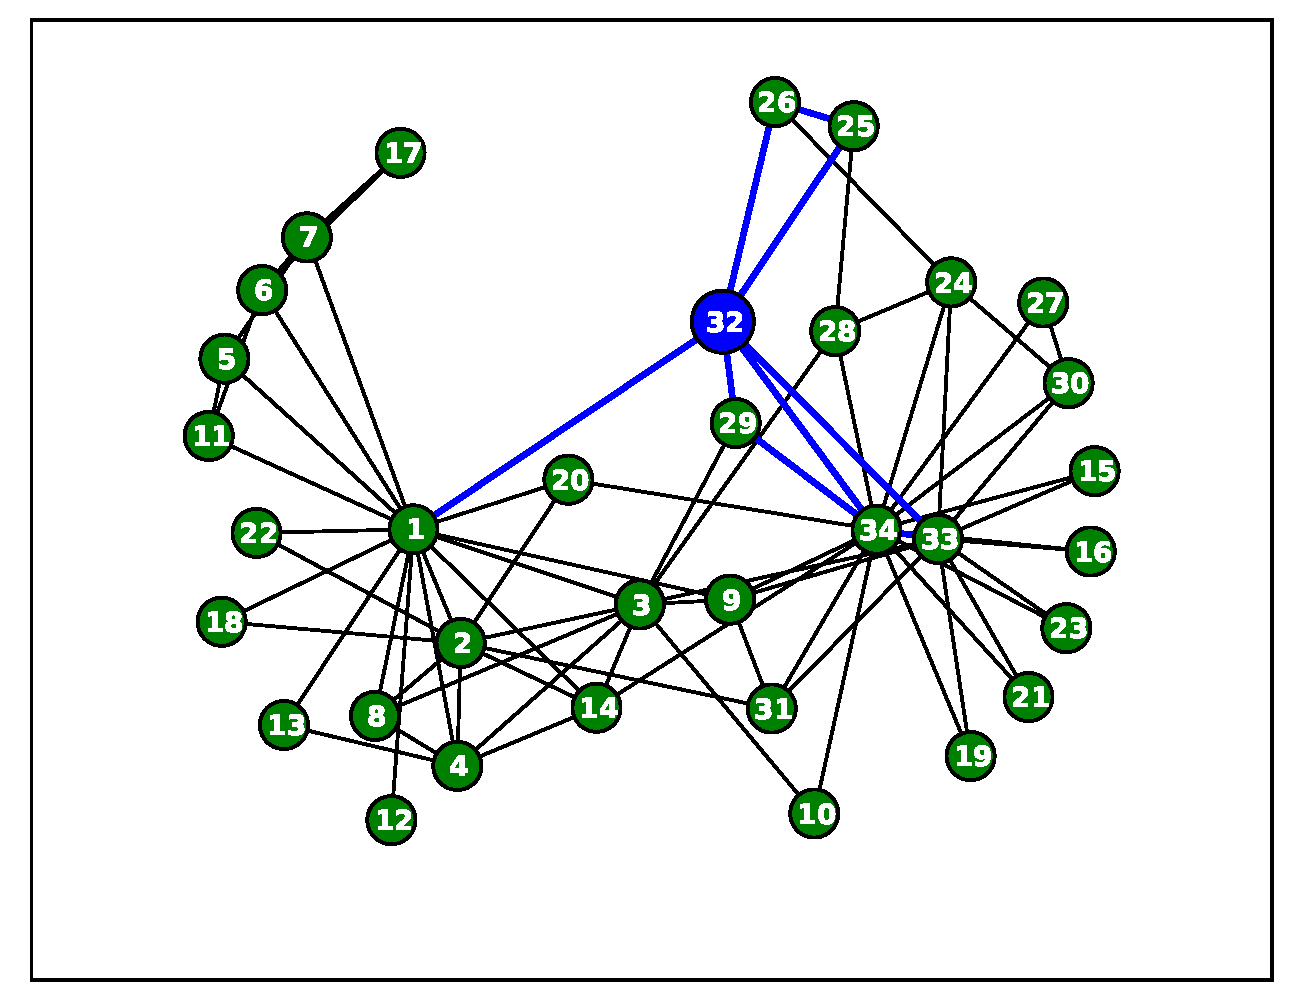
\includegraphics[scale=0.36]{./chap5/SD1}}
%	%\hspace{3em}%
%	\subcaptionbox{节点32邻居知道某个信息的环境\label{fig:chap05SD2}}
%	{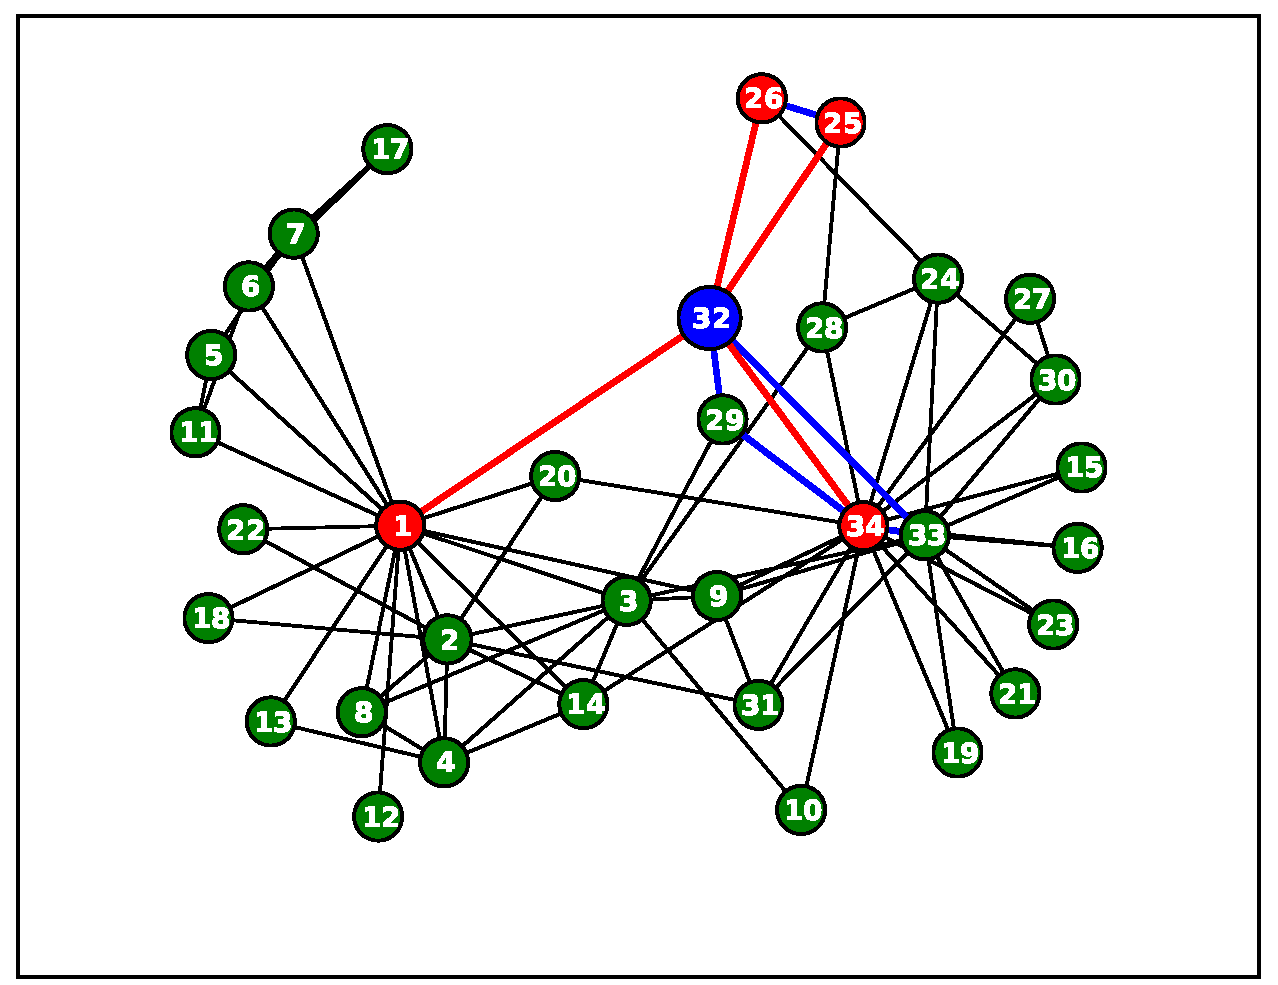
\includegraphics[scale=0.36]{./chap5/SD2}}
%	
%	\caption{以Zachary俱乐部网络为例,节点32,接受不同圈子信息的多样性结构}
%	\label{fig:chap05egonetwork}
%\end{figure}
%我们以节点[32]作为信息的接收点,如图~\ref{fig:chap05SD2}所示,你同时从你研究生同学节点[25,26]分别得到一信息,其可信度与你分别从高中同学[1]和大学同学[34]得到一消息是完全不同的,你对后一种情况下信息的可信性和感兴趣程度将倍增,你转发传播该信息的概率将会累积增加。

下面实验,我们即考虑节点自身属性,特别考虑了信息传播过程中节点所处结构多样性的外部环境因素。应用现实实际数据集Netsceince网络、Email网络、Blogs网络,数据具体描述参考表~\ref{dataset-statistics},Netscience网络和Email网络的节点度的幂律分布情况,如图~\ref{fig:chap05netsciencePowerlaw}、~\ref{fig:chap05emailPowerlaw}所示。Blogs网络的节点度的幂律分布情况,见第四章节图~\ref{fig:chap4BlogsPowerlaw}所示。
\begin{figure}[H]
	\centering%
	\subcaptionbox{Netscience数据\cite{boccaletti2006complex},其中节点数为379,边数为914\label{fig:chap05netsciencePowerlaw}}
	%标题的长度,超过则会换行,如下一个小图。
	{\includegraphics[width=7.3cm]{./chap5/netsciencePowerlaw}}
	%\hspace{3em}%
	\subcaptionbox{Email数据\cite{guimera2003self},其中节点数为1133,边数为5451\label{fig:chap05emailPowerlaw}}
	{\includegraphics[width=7.3cm]{./chap5/emailPowerlaw}}
	
	\caption{Netscience、Email网络的度分布情况}
\end{figure}


%\begin{figure}[H]
%	\centering
%	\includegraphics[scale=0.5]{./chap5/blogsPowerlaw}
%	\caption{Blogs数据\cite{xie2006social},其中节点数为3982,边数为6803}
%	\label{fig:chap05blogsPowerlaw}
%\end{figure}

我们采用影响力最大化的典型算法DegreeHeuristic算法\cite{kempe2003maximizing},对ISSD模型与IC模型、LT模型进行了分析比较,在IC模型实验模拟传播过程中,每次选取传播种子节点$1 \leq k \leq 30$作为传播源的种子集合,传播概率取$p=0.01$。三种模型传播范围取10000次迭代求均值,横轴为根据各算法中传播影响最大节点进行排序所得的集合大小,纵轴为在选取相应传播种子节点集合条件下的传播范围大小。

\begin{figure}[H]
	\centering%
	\subcaptionbox{Netscience数据\cite{boccaletti2006complex},其中节点数为379,边数为914\label{fig:chap05netscienceDiffModelCampare}}
	%标题的长度,超过则会换行,如下一个小图。
	{\includegraphics[width=7.3cm]{./chap5/netscienceDiffModelCampare}}
	%\hspace{3em}%
	\subcaptionbox{Email数据\cite{guimera2003self},其中节点数为1133,边数为5451\label{fig:chap05emailDiffModelCampare}}
	{\includegraphics[width=7.3cm]{./chap5/emailDiffModelCampare}}
	
	\caption{ISSD模型与IC、LT模型运行DegreeHeuristic算法结果比较}
\end{figure}

%\begin{figure}[H]
%	\centering
%	\includegraphics[scale=0.5]{./chap5/netscienceDiffModelCampare}
%	\caption{Netscience数据\cite{xie2006social},其中节点数为379,边数为914}
%	\label{fig:chap05netscienceDiffModelCampare}
%\end{figure}
%
%\begin{figure}[H]
%	\centering
%	\includegraphics[scale=0.5]{./chap5/emailDiffModelCampare}
%	\caption{Email数据\cite{xie2006social},其中节点数为1133,边数为5451}
%	\label{fig:chap05emailDiffModelCampare}
%\end{figure}
从图~\ref{fig:chap05netscienceDiffModelCampare}与图~\ref{fig:chap05emailDiffModelCampare},我们可以看到DegreeHeuristic算法在IC模型与LT模型运行结果相似,随着种子节点的加入,影响力逐步增加,曲线变化趋势相对较稳定。而算法运行结果在ISSD模型中出现波动,随着种子节点的增加,影响力范围反而减少现象,这与我们前面在悲惨世界网络中看到的现象相符。利用已有的IC模型和LT模型对复杂的信息传播过程进行分析是不完全的,而我们所提出ISSD模型特别针对信息传播考虑了节点自身因素、外部环境特点及时间因素等,对于分析信息传播更加具有针对性,为信息传播这个热点和难点问题提供了新模型,为探索信息传播规律打下了基础,希望能对各研究领域给予启发。

\section{影响力最大化算法}

\subsection{KClique Heuristic算法}
现实社会中信息总是在各类社交圈中传播,人们总是由于成长阶段、工作学习、兴趣爱好、生活地域等原因,形成一个又一个关系紧密的社交圈。这与我们社交网络形成的网络关系基本相符,你会有班级同学圈,工作同事圈,娱乐伙伴圈等等社交圈,你认识的这些人,他们之间也很可能都相互认识,也可能不认识。从你的角度来看,你是联系这些人的Ego节点。,我们认为最具有影响力的节点是能最大化联系整个社交网络,跨越多个圈子的人,类似于整个复杂网络中的结构洞(Structural holes)\cite{walker1997social,ahuja2000collaboration,burt2009structural},对于这些圈子中有重叠社区划分是研究信息传播的关键基础。
有重叠社区划分最早是由G.Palla等人2005年在《Nature》中提出K-clique社区划分算法CMP\cite{palla2005uncovering},他们定义社区内的任意节点应与多数节点连接,即一个社区可以表示为多个子图的并集,子图要求其内部节点之间必须有联系。在数学上定义一个完全连接的全连接图为K-clique,其中$K$为节点的数目,邻接K-clique是指两个K-clique至少共享$k-1$个节点。简单举例描述如图~\ref{fig:chap05CliqueExample}所示。
\begin{figure}[H]
	\centering%
	\subcaptionbox{K-clique网络关系例图\label{fig:chap05CliqueExample1}}
	%标题的长度,超过则会换行,如下一个小图。
	{\includegraphics[width=7.3cm]{./chap5/CliqueExample1}}
	%\hspace{3em}%
	\subcaptionbox{K-clique网络关系例图中K=3的部分社区划分\label{fig:chap05CliqueExample2}}
	{\includegraphics[width=7.3cm]{./chap5/CliqueExample2}}
	
	\caption{K-clique社区网络划分图例}
	\label{fig:chap05CliqueExample}
\end{figure}
我们提出的KClique Heuristic算法的基本思路是:首先对整个社交网络进行K-clique划分,然后找出Top-K个在所有有重叠划分的社区中出现次数最多的节点集合。其中K是控制社区内部紧密程度的参数。具体描述如算法~\ref{KCliqueHeuristic}所示:
\begin{algorithm}
	\caption{KCliqueHeuristic(G,s)}
	\label{KCliqueHeuristic}
	\begin{algorithmic}[1]
		\STATE initialize $S = \phi$,$dict =\{ \} $
		\STATE KC = KCliqueCommunity(G,k)
		\FOR {each vertex $v \in V$}
		\FOR {each clique $kc_i \in KC$}
		\IF {$v \in kc_i$}
		\STATE dict[v] += 1
		\ENDIF
		\ENDFOR
		\ENDFOR
		\STATE  $S$ = argmaxTop(dict[v])[1:s]
		\RETURN $S$
	\end{algorithmic}
\end{algorithm}

应用第~\ref{cha:4thChap04}章所提到的相关算法,与我们提出的KClique Heuristic算法,在IC模型、LT模型及ISSD模型中进行了影响力最大化实验比较。在IC模型模拟传播过程中,我们主要分析了传播概率较小的情况,节点传播概率p=0.01时传播过程的运行效果及时间。

\begin{figure}[H]
	\centering%
	\subcaptionbox{Blogs网络\label{fig:BlogsDiifAlgIISSDclique}}
	%标题的长度,超过则会换行,如下一个小图。
	{\includegraphics[width=7.3cm]{./chap5/BlogsDiifAlgIISSDclique}}
	%\hspace{3em}%
	\subcaptionbox{Netscience网络\label{fig:netscienceDiifAlgISSDclique}}
	{\includegraphics[width=7.3cm]{./chap5/netscienceDiifAlgISSDclique}}
	
	\caption{ISSD模型下不同算法运行结果分析比较}
\end{figure}

\begin{figure}[H]
	\centering%
	\subcaptionbox{Blogs网络\label{fig:BlogsDiifAlgICclique}}
	%标题的长度,超过则会换行,如下一个小图。
	{\includegraphics[width=7.3cm]{./chap5/BlogsDiifAlgICclique}}
	%\hspace{3em}%
	\subcaptionbox{Netscience网络\label{fig:NetscienceDiifAlgICclique}}
	{\includegraphics[width=7.3cm]{./chap5/NetscienceDiifAlgICclique}}
	
	\caption{IC模型下不同算法运行结果分析比较}
\end{figure}

\begin{figure}[H]
	\centering%
	\subcaptionbox{Blogs网络\label{fig:BlogsDiifAlgLTclique}}
	%标题的长度,超过则会换行,如下一个小图。
	{\includegraphics[width=7.3cm]{./chap5/BlogsDiifAlgLTclique}}
	%\hspace{3em}%
	\subcaptionbox{Netscience网络\label{fig:NetscienceDiifAlgLTclique}}
	{\includegraphics[width=7.3cm]{./chap5/NetscienceDiifAlgLTclique}}
	
	\caption{LT模型下不同算法运行结果分析比较}
\end{figure}

从图~\ref{fig:BlogsDiifAlgIISSDclique}到图~\ref{fig:netscienceDiifAlgISSDclique},可以看出我们所提出的KClique Heuristic算法,在ISSD模型中运行效果要好于其它算法,且在IC模型与LT模型中运行效果也与其它算法相似。通过实验,可以看出我们的模型同样可以应用于其他类型的复杂网络中,同时算法适应性较好。与算法设想:最具有影响力的节点是那些能最大化联系整个社交网络社区的节点基本一致。

\subsection{Community Leader Heuristic算法}%说明算法communityDegree,
%Lesmis diff community alg graph
常言道“物以类聚,人以群分”,对于无重叠社区划分所遵循的常理是社区内节点联系紧密,而社区之间联系松散。通常人们更加相信关系紧密的圈内信息,而不是其它圈外其他来源的信息。这里以《悲惨世界》人物关系网络为例进行说明。如图~\ref{fig:chap05lesmis}所示,主要人物是,主人公Jean Valjean(冉阿让),探长Javert(贾维),神父Bishop Myriel(米里哀),Eponine(爱潘妮),女工Fantine(芳汀)及其女儿Cosette(珂赛特)。如何仅仅从节点关系度来划分,这与作者小说想描述的人物重点是有出入的,如Eponine(爱潘妮)的弟弟Gavroche(加夫罗契)就比Myriel(米里哀)联系人要多,也就是度数要大。即所以传统以节点度数作为影响力最大化的方法是存在一定的缺陷的。
\begin{figure}[H]
	\centering
	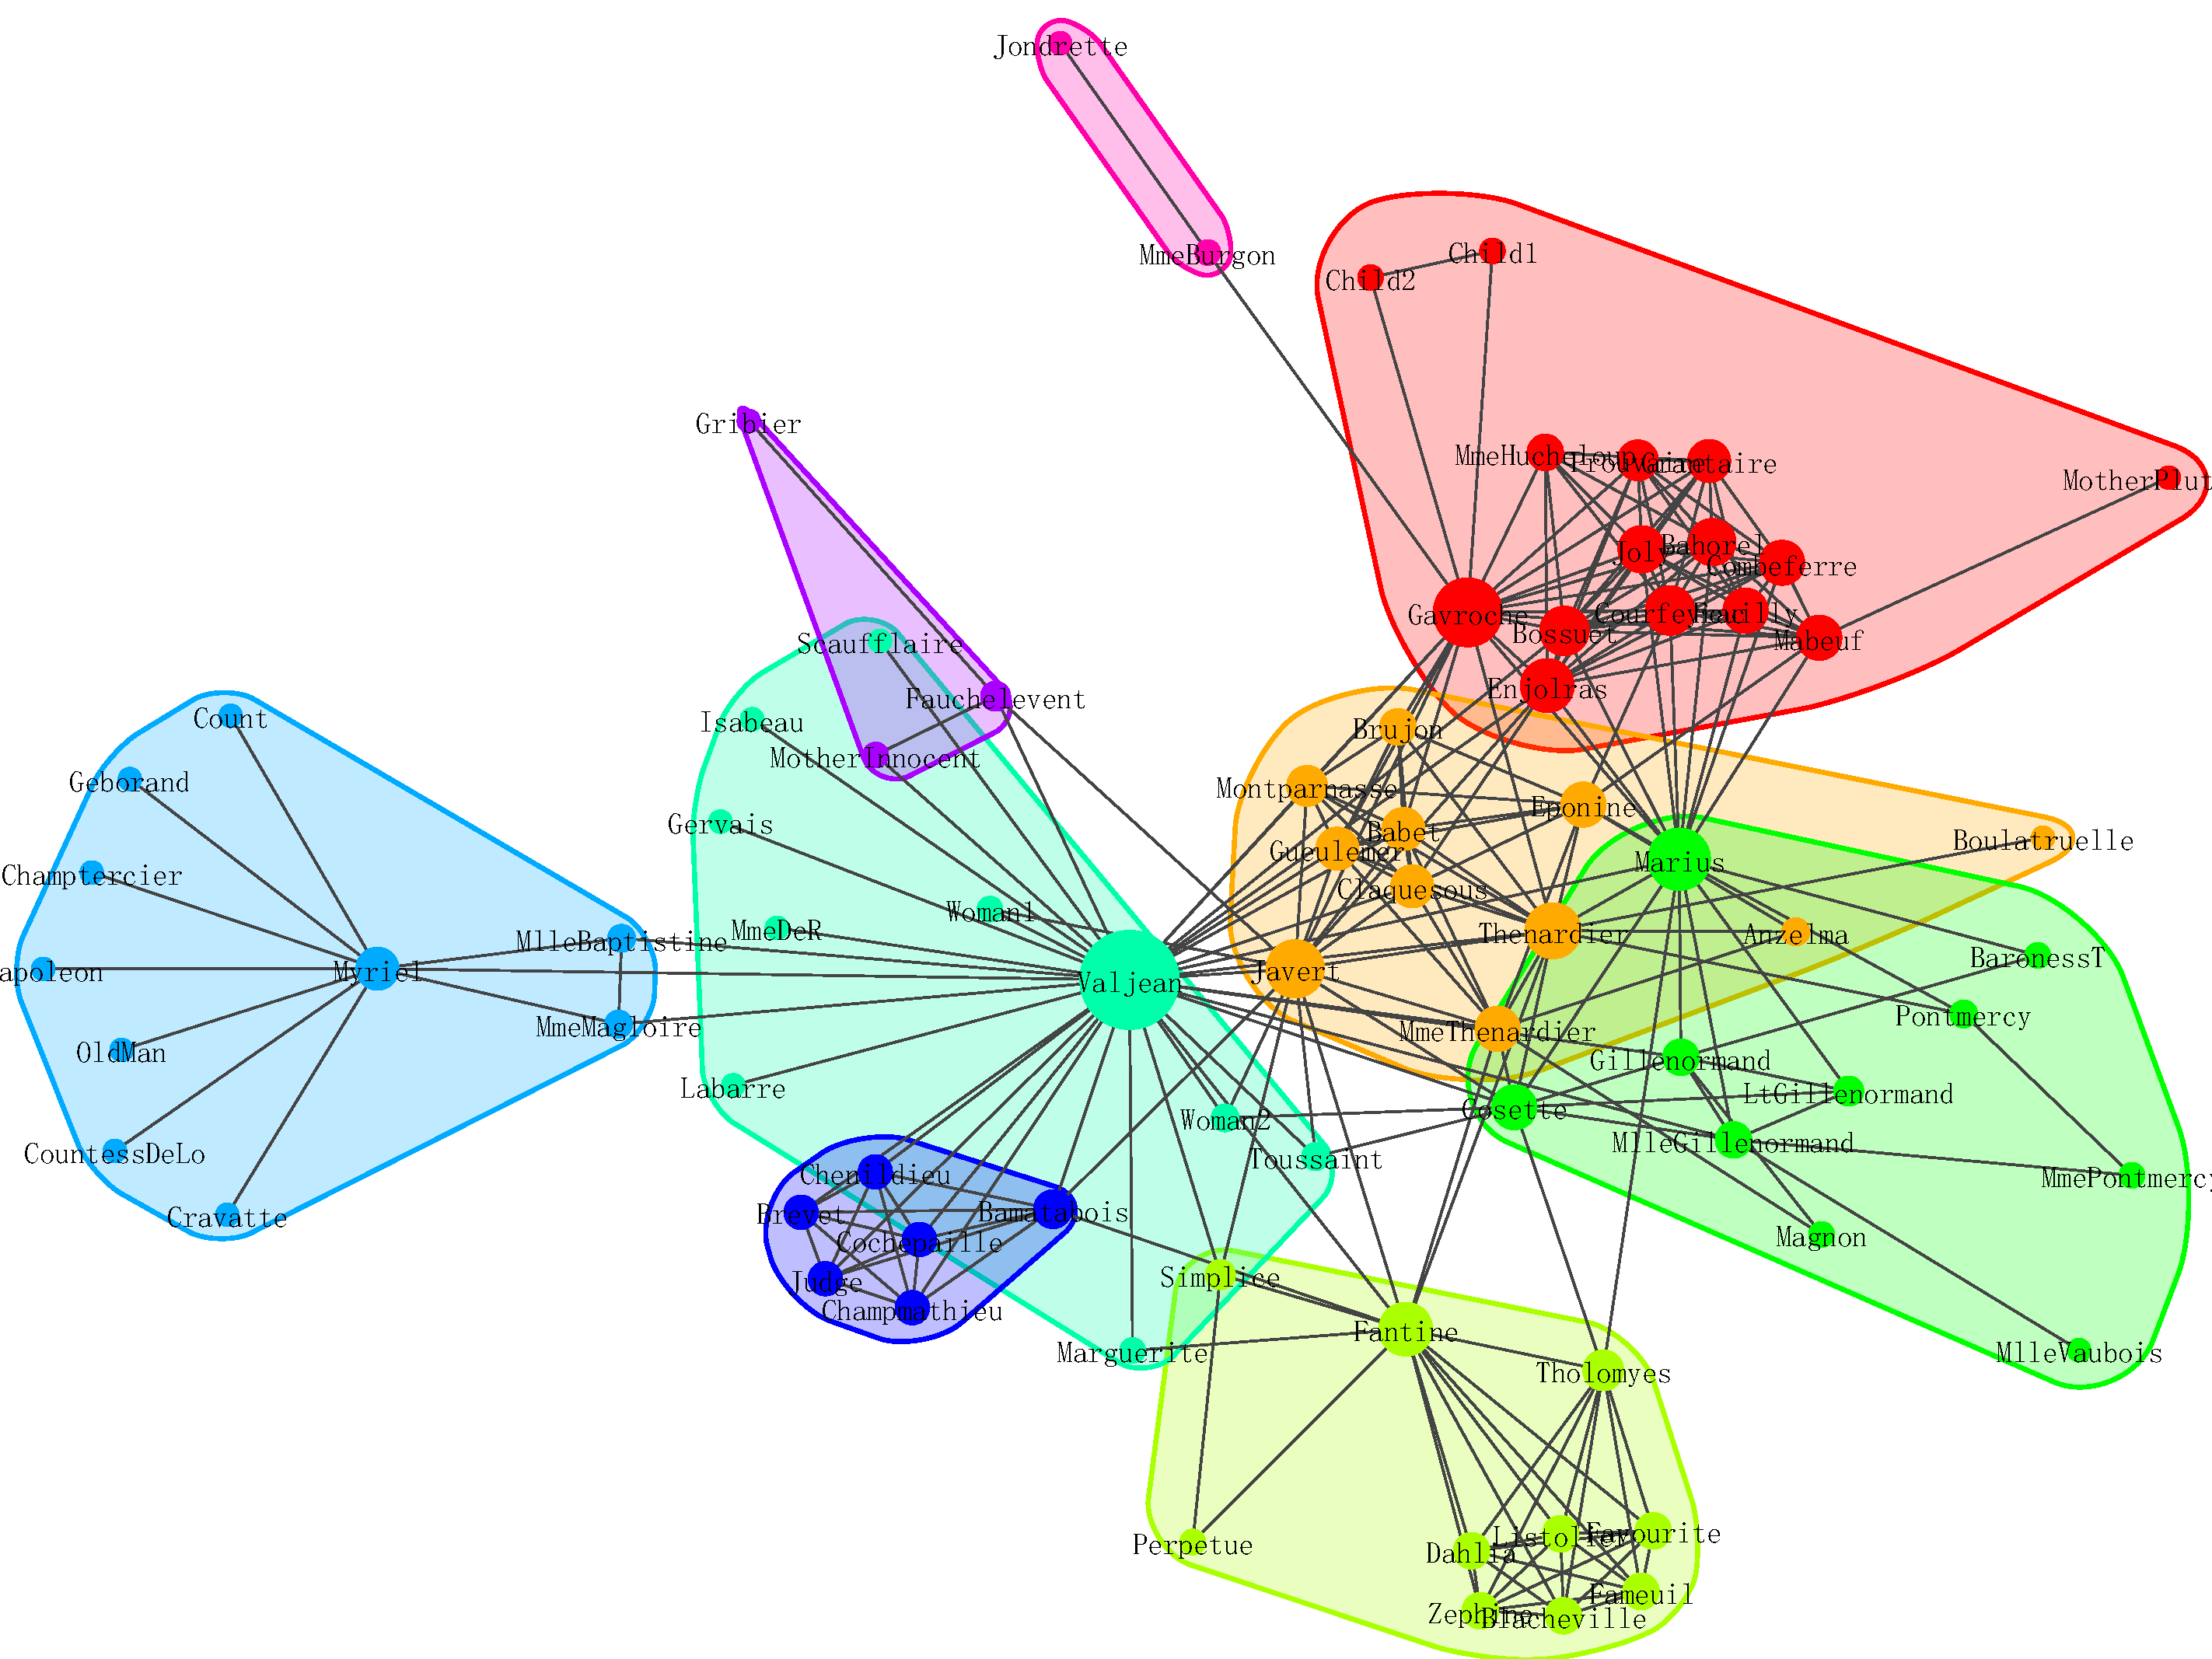
\includegraphics[scale=0.45]{./chap5/lesmis-info}
	\caption{Infomaps算法\cite{rosvall2008maps}社区划分悲惨世界人物关系网络图}
	\label{fig:chap05lesmis}
\end{figure}
另一方面,目前分析信息传播过程都以个体或节点为单位粒度进行分析,而现实社交网络中注册用户一般都在$10^8$以上,用户关系网络复杂。如果特别是针对整个用户进行敏感信息监管几乎是不可能的。我们知道论坛、微博中普遍存在少数活跃用户推动大多数信息的传播,就是少数用户与多数用户有交互联系,20/80原理同样存在于社交网络上的信息传播规律。
针对此类问题我们提出了社区意见领袖启发式(Community Leader Heuristic)CLH模型,
从每一个社区中选择意见领袖\cite{katz1957two}作为传播节点,模型示意图如图~\ref{fig:chap05communtyLeaderToNode}所示。每个社区内的意见领袖的可信度要高于社区处人员,意见领袖的选择有利于信息的传播。
\begin{figure}[H]
	\centering
	\includegraphics[scale=0.45]{./chap5/chap05communtyLeaderToNode}
	\caption{社区意见领袖启发式算法示意图}
	\label{fig:chap05communtyLeaderToNode}
\end{figure}
我们可以根据不同的需求,对网络进行划分成不同层次的网络社区。通过CLH模型分析图~\ref{fig:chap05communtyLeaderToNode},可以得到社区意见领袖节点[4,7,9,14],我们也可以进一步计算划分[4,7,9,14],得出新粒度的意见领袖为节点[9]。从相反的角度分析,可以在大社团中再次划分成多个小的社团,从每个小社团中发现其意见领袖,以小粒度分析信息传播过程。如图~\ref{fig:Chap05blogsCommunityToNode}所示,对Blogs网络中$n=3982$个节点,$m=6803$条边以无重叠社区划分的新粒度网络关系图。这样我们可以从中观层次了解整个网络关系,了解信息如何在社区(圈子)内传播,而不至于陷入庞大、不可视的复杂关系中,从而可为信息监控提供依据。
\begin{figure}[H]
	\centering
	\includegraphics[scale=0.50]{./chap5/Chap05blogsCommunityToNode}
	\caption{Blogs网络根据CLH形成的新网络关系图}
	\label{fig:Chap05blogsCommunityToNode}
\end{figure}
因此可以根据实际需要划分成不同粒度的信息传播模型,或信息监控对象。这个常理与我们现实生活中的行政区域化分及行政区域的行政领导的模式相似,目前很多广告也是根据不同的地区,选择不同的区域名人做广告。

我们应用CLH模型到影响力最大化问题中,社区意见领袖启发式(Community Leader Heuristic)CLH算法如下:
\begin{algorithm}
	\caption{communtiyLeaderHeuristic(G,k)}
	\label{communityIM}
	\begin{algorithmic}[1]
		\STATE initialize $S = \phi$
		\STATE $C=communtiyDetect(G)$
		\FOR {each community $c_i \in C$}
		\STATE $subGraph_{i}$ = $k * c_i/n$
		\STATE $subC_i = communtiyDetect(subGraph_{i})$
		\FOR {each subCommunity $c_j \in subC_i $}
		\STATE select $s_{leader}$ = argmaxLeader($c_j$)
		\STATE $S = S \cup s_{leader} $ 
		\ENDFOR
		\ENDFOR
		\RETURN $S$
	\end{algorithmic}
\end{algorithm}

我们应用章节~\ref{cha:4thChap04}所提出的相关算法,与我们提出的KClique Heuristic算法、CLH算法,在~\ref{cha:secondChap02}中所提到的IC模型、LT模型及我们所提出的ISSD模型,对我们所提出的算法及模型进行了最大影响力最大化算法分析比较。在IC模型模拟传播过程中,我们主要分析了传播概率较小的情况,节点传播概率p=0.01(如果节点的传播能力很强,很难区分单个个体的重要性)时传播过程的运行效果及时间。
数据集我们采用Blogs网络和email网络数据。
\begin{figure}[H]
	\centering%
	\subcaptionbox{Blogs网络\label{fig:BlogsDiifAlgIISSDclt}}
	%标题的长度,超过则会换行,如下一个小图。
	{\includegraphics[width=7.3cm]{./chap5/BlogsDiifAlgIISSDclt}}
	%\hspace{3em}%
	\subcaptionbox{Netscience网络\label{fig:netscienceDiifAlgISSD}}
	{\includegraphics[width=7.3cm]{./chap5/netscienceDiifAlgISSD}}
	
	\caption{ISSD模型下不同算法运行结果分析比较}
\end{figure}

\begin{figure}[H]
	\centering%
	\subcaptionbox{Blogs网络\label{fig:BlogsDiifAlgICLT}}
	%标题的长度,超过则会换行,如下一个小图。
	{\includegraphics[width=7.3cm]{./chap5/BlogsDiifAlgICLT}}
	%\hspace{3em}%
	\subcaptionbox{Email网络\label{fig:NetscienceDiifAlgICLT}}
	{\includegraphics[width=7.3cm]{./chap5/NetscienceDiifAlgICLT}}
	
	\caption{IC模型下不同算法运行结果分析比较}
\end{figure}

\begin{figure}[H]
	\centering%
	\subcaptionbox{Blogs网络\label{fig:BlogsDiifAlgLTCLT}}
	%标题的长度,超过则会换行,如下一个小图。
	{\includegraphics[width=7.3cm]{./chap5/BlogsDiifAlgLTCLT}}
	%\hspace{3em}%
	\subcaptionbox{Netscience网络\label{fig:NetscienceDiifAlgLTCLT}}
	{\includegraphics[width=7.3cm]{./chap5/NetscienceDiifAlgLTCLT}}
	
	\caption{LT模型下不同算法运行结果分析比较}
\end{figure}

从图~\ref{fig:BlogsDiifAlgIISSDclt}到图~\ref{fig:netscienceDiifAlgISSD},可以看出我们所提出的CLT算法、KClique Heuristic算法,在ISSD模型中运行效果要好于已有算法,且在IC模型与LT模型中运行效果也与经典算法相似。这与我们的算法思路:每个社区内的意见领袖更有利于信息传播相符。而且CLT算法可以根据实际需要从不同的粒度进行信息传播,能更好适用于信息监控。

\section{本章小结}
在本章中,我们深入研究了信息传播过程,分析了信息传播随时间变化特点,并参照“牛顿冷却定律”提出了适应信息传播的时间变化模型。同时考虑了接收信息个体自身内部属性及所在Ego网络中传播信息状态这一外部属性,按照其与传播信息邻居的关系紧密程度从连通性,无重叠社区,K-truesses子图,有重叠社区Kclique子图等4种结构多样性特点进行了分析。我们给出了符合信息传播的5个假设;给出了信息传播机理,即信息传播过程中未知信息状态(\underline{\textbf{U}}nknown)、得知信息状态(\underline{\textbf{K}}nown)、传播信息状态(\underline{\textbf{A}}pproved)和信息疲惫态(\underline{\textbf{E}}xhausted)等4种信息传播状态类型;提出了ISSD信息传播结构多样化模型,并对整个变化过程的进行了形式化定义和描述。实验分析了信息传播过程中时间影响、结构多样化影响特点。最后,我们结合前面影响力最大化方法,提出了符合信息传播的两个最大化算法,KClique Heuristic算法和CLH算法。实验证明两个算法不但在ISSD模型中效果突出,而且同样也适用于IC模型与LT模型,运行效果与经典算法相似,说明了算法的通用性和适用性。总之,ISSD模型的提出使人们分析信息传播过程及阶段状态有了清晰的认识,并可以进行量化,这方便了信息传播过程的理论研究。希望能在疾病预防、网络安全、市场营销、广告投放、舆情分析、信息监控等实际热点领域中得以应用,期望能给相关研究人员给予启发。
%同时我们的模型也可成为重要热点人物发现,热点团体发现的研究基础。这为信息的研究提供了新的思路和方法。